\documentclass[twoside]{book}

% Packages required by doxygen
\usepackage{fixltx2e}
\usepackage{calc}
\usepackage{doxygen}
\usepackage[export]{adjustbox} % also loads graphicx
\usepackage{graphicx}
\usepackage[utf8]{inputenc}
\usepackage{makeidx}
\usepackage{multicol}
\usepackage{multirow}
\PassOptionsToPackage{warn}{textcomp}
\usepackage{textcomp}
\usepackage[nointegrals]{wasysym}
\usepackage[table]{xcolor}

% Font selection
\usepackage[T1]{fontenc}
\usepackage[scaled=.90]{helvet}
\usepackage{courier}
\usepackage{amssymb}
\usepackage{sectsty}
\renewcommand{\familydefault}{\sfdefault}
\allsectionsfont{%
  \fontseries{bc}\selectfont%
  \color{darkgray}%
}
\renewcommand{\DoxyLabelFont}{%
  \fontseries{bc}\selectfont%
  \color{darkgray}%
}
\newcommand{\+}{\discretionary{\mbox{\scriptsize$\hookleftarrow$}}{}{}}

% Page & text layout
\usepackage{geometry}
\geometry{%
  a4paper,%
  top=2.5cm,%
  bottom=2.5cm,%
  left=2.5cm,%
  right=2.5cm%
}
\tolerance=750
\hfuzz=15pt
\hbadness=750
\setlength{\emergencystretch}{15pt}
\setlength{\parindent}{0cm}
\setlength{\parskip}{3ex plus 2ex minus 2ex}
\makeatletter
\renewcommand{\paragraph}{%
  \@startsection{paragraph}{4}{0ex}{-1.0ex}{1.0ex}{%
    \normalfont\normalsize\bfseries\SS@parafont%
  }%
}
\renewcommand{\subparagraph}{%
  \@startsection{subparagraph}{5}{0ex}{-1.0ex}{1.0ex}{%
    \normalfont\normalsize\bfseries\SS@subparafont%
  }%
}
\makeatother

% Headers & footers
\usepackage{fancyhdr}
\pagestyle{fancyplain}
\fancyhead[LE]{\fancyplain{}{\bfseries\thepage}}
\fancyhead[CE]{\fancyplain{}{}}
\fancyhead[RE]{\fancyplain{}{\bfseries\leftmark}}
\fancyhead[LO]{\fancyplain{}{\bfseries\rightmark}}
\fancyhead[CO]{\fancyplain{}{}}
\fancyhead[RO]{\fancyplain{}{\bfseries\thepage}}
\fancyfoot[LE]{\fancyplain{}{}}
\fancyfoot[CE]{\fancyplain{}{}}
\fancyfoot[RE]{\fancyplain{}{\bfseries\scriptsize Generated by Doxygen }}
\fancyfoot[LO]{\fancyplain{}{\bfseries\scriptsize Generated by Doxygen }}
\fancyfoot[CO]{\fancyplain{}{}}
\fancyfoot[RO]{\fancyplain{}{}}
\renewcommand{\footrulewidth}{0.4pt}
\renewcommand{\chaptermark}[1]{%
  \markboth{#1}{}%
}
\renewcommand{\sectionmark}[1]{%
  \markright{\thesection\ #1}%
}

% Indices & bibliography
\usepackage{natbib}
\usepackage[titles]{tocloft}
\setcounter{tocdepth}{3}
\setcounter{secnumdepth}{5}
\makeindex

% Hyperlinks (required, but should be loaded last)
\usepackage{ifpdf}
\ifpdf
  \usepackage[pdftex,pagebackref=true]{hyperref}
\else
  \usepackage[ps2pdf,pagebackref=true]{hyperref}
\fi
\hypersetup{%
  colorlinks=true,%
  linkcolor=blue,%
  citecolor=blue,%
  unicode%
}

% Custom commands
\newcommand{\clearemptydoublepage}{%
  \newpage{\pagestyle{empty}\cleardoublepage}%
}

\usepackage{caption}
\captionsetup{labelsep=space,justification=centering,font={bf},singlelinecheck=off,skip=4pt,position=top}

%===== C O N T E N T S =====

\begin{document}

% Titlepage & ToC
\hypersetup{pageanchor=false,
             bookmarksnumbered=true,
             pdfencoding=unicode
            }
\pagenumbering{alph}
\begin{titlepage}
\vspace*{7cm}
\begin{center}%
{\Large Aurora \\[1ex]\large 0.\+1 }\\
\vspace*{1cm}
{\large Generated by Doxygen 1.8.13}\\
\end{center}
\end{titlepage}
\clearemptydoublepage
\pagenumbering{roman}
\tableofcontents
\clearemptydoublepage
\pagenumbering{arabic}
\hypersetup{pageanchor=true}

%--- Begin generated contents ---
\chapter{Aurora headers}
\label{index}\hypertarget{index}{}{\bfseries \hyperlink{_snd_base_8h}{Snd\+Base.\+h}}\+: base class and utilities

{\bfseries \hyperlink{_osc_8h}{Osc.\+h}}\+: generic oscillator and synthesis function templates

{\bfseries \hyperlink{_bl_osc_8h}{Bl\+Osc.\+h}}\+: bandlimited oscillator

{\bfseries \hyperlink{_env_8h}{Env.\+h}}\+: generic envelope and function templates

{\bfseries \hyperlink{_f_f_t_8h}{F\+F\+T.\+h}}\+: fast-\/fourier transform

{\bfseries \hyperlink{_four_pole_8h}{Four\+Pole.\+h}}\+: four-\/pole lowpass filter

{\bfseries \hyperlink{_func_8h}{Func.\+h}}\+: generic function maps 
\chapter{Namespace Index}
\section{Namespace List}
Here is a list of all namespaces with brief descriptions\+:\begin{DoxyCompactList}
\item\contentsline{section}{\hyperlink{namespace_aurora}{Aurora} }{\pageref{namespace_aurora}}{}
\end{DoxyCompactList}

\chapter{Hierarchical Index}
\section{Class Hierarchy}
This inheritance list is sorted roughly, but not completely, alphabetically\+:\begin{DoxyCompactList}
\item \contentsline{section}{Aurora\+:\+:F\+FT$<$ S $>$}{\pageref{class_aurora_1_1_f_f_t}}{}
\item \contentsline{section}{Aurora\+:\+:IR$<$ S $>$}{\pageref{class_aurora_1_1_i_r}}{}
\item \contentsline{section}{Aurora\+:\+:Snd\+Base$<$ S $>$}{\pageref{class_aurora_1_1_snd_base}}{}
\begin{DoxyCompactList}
\item \contentsline{section}{Aurora\+:\+:Bin\+Op$<$ S, OP $>$}{\pageref{class_aurora_1_1_bin_op}}{}
\item \contentsline{section}{Aurora\+:\+:Buff$<$ S $>$}{\pageref{class_aurora_1_1_buff}}{}
\item \contentsline{section}{Aurora\+:\+:Conv$<$ S $>$}{\pageref{class_aurora_1_1_conv}}{}
\item \contentsline{section}{Aurora\+:\+:Del$<$ S, FN $>$}{\pageref{class_aurora_1_1_del}}{}
\item \contentsline{section}{Aurora\+:\+:Env$<$ S, FN $>$}{\pageref{class_aurora_1_1_env}}{}
\item \contentsline{section}{Aurora\+:\+:Eq$<$ S $>$}{\pageref{class_aurora_1_1_eq}}{}
\item \contentsline{section}{Aurora\+:\+:Fil$<$ S, CF, FN $>$}{\pageref{class_aurora_1_1_fil}}{}
\item \contentsline{section}{Aurora\+:\+:Four\+Pole$<$ S $>$}{\pageref{class_aurora_1_1_four_pole}}{}
\item \contentsline{section}{Aurora\+:\+:Func$<$ S, FN $>$}{\pageref{class_aurora_1_1_func}}{}
\item \contentsline{section}{Aurora\+:\+:Mix$<$ S $>$}{\pageref{class_aurora_1_1_mix}}{}
\item \contentsline{section}{Aurora\+:\+:One\+Pole$<$ S $>$}{\pageref{class_aurora_1_1_one_pole}}{}
\item \contentsline{section}{Aurora\+:\+:Osc$<$ S, FN $>$}{\pageref{class_aurora_1_1_osc}}{}
\begin{DoxyCompactList}
\item \contentsline{section}{Aurora\+:\+:Bl\+Osc$<$ S, FN $>$}{\pageref{class_aurora_1_1_bl_osc}}{}
\end{DoxyCompactList}
\item \contentsline{section}{Aurora\+:\+:Two\+Pole$<$ S, FN $>$}{\pageref{class_aurora_1_1_two_pole}}{}
\end{DoxyCompactList}
\item \contentsline{section}{Aurora\+:\+:Table\+Set$<$ S $>$}{\pageref{class_aurora_1_1_table_set}}{}
\end{DoxyCompactList}

\chapter{Class Index}
\section{Class List}
Here are the classes, structs, unions and interfaces with brief descriptions\+:\begin{DoxyCompactList}
\item\contentsline{section}{\hyperlink{class_aurora_1_1_bin_op}{Aurora\+::\+Bin\+Op$<$ S $>$} }{\pageref{class_aurora_1_1_bin_op}}{}
\item\contentsline{section}{\hyperlink{class_aurora_1_1_bl_osc}{Aurora\+::\+Bl\+Osc$<$ S $>$} }{\pageref{class_aurora_1_1_bl_osc}}{}
\item\contentsline{section}{\hyperlink{class_aurora_1_1_env}{Aurora\+::\+Env$<$ S $>$} }{\pageref{class_aurora_1_1_env}}{}
\item\contentsline{section}{\hyperlink{class_aurora_1_1_f_f_t}{Aurora\+::\+F\+F\+T$<$ S $>$} }{\pageref{class_aurora_1_1_f_f_t}}{}
\item\contentsline{section}{\hyperlink{class_aurora_1_1_four_pole}{Aurora\+::\+Four\+Pole$<$ S $>$} }{\pageref{class_aurora_1_1_four_pole}}{}
\item\contentsline{section}{\hyperlink{class_aurora_1_1_osc}{Aurora\+::\+Osc$<$ S $>$} }{\pageref{class_aurora_1_1_osc}}{}
\item\contentsline{section}{\hyperlink{class_aurora_1_1_snd_base}{Aurora\+::\+Snd\+Base$<$ S $>$} }{\pageref{class_aurora_1_1_snd_base}}{}
\item\contentsline{section}{\hyperlink{class_aurora_1_1_table_set}{Aurora\+::\+Table\+Set$<$ S $>$} }{\pageref{class_aurora_1_1_table_set}}{}
\end{DoxyCompactList}

\chapter{File Index}
\doxysection{File List}
Here is a list of all files with brief descriptions\+:\begin{DoxyCompactList}
\item\contentsline{section}{\mbox{\hyperlink{_bl_osc_8h}{Bl\+Osc.\+h}} }{\pageref{_bl_osc_8h}}{}
\item\contentsline{section}{\mbox{\hyperlink{_conv_8h}{Conv.\+h}} }{\pageref{_conv_8h}}{}
\item\contentsline{section}{\mbox{\hyperlink{_del_8h}{Del.\+h}} }{\pageref{_del_8h}}{}
\item\contentsline{section}{\mbox{\hyperlink{_env_8h}{Env.\+h}} }{\pageref{_env_8h}}{}
\item\contentsline{section}{\mbox{\hyperlink{_eq_8h}{Eq.\+h}} }{\pageref{_eq_8h}}{}
\item\contentsline{section}{\mbox{\hyperlink{_f_f_t_8h}{FFT.\+h}} }{\pageref{_f_f_t_8h}}{}
\item\contentsline{section}{\mbox{\hyperlink{_fil_8h}{Fil.\+h}} }{\pageref{_fil_8h}}{}
\item\contentsline{section}{\mbox{\hyperlink{_four_pole_8h}{Four\+Pole.\+h}} }{\pageref{_four_pole_8h}}{}
\item\contentsline{section}{\mbox{\hyperlink{_func_8h}{Func.\+h}} }{\pageref{_func_8h}}{}
\item\contentsline{section}{\mbox{\hyperlink{_one_pole_8h}{One\+Pole.\+h}} }{\pageref{_one_pole_8h}}{}
\item\contentsline{section}{\mbox{\hyperlink{_osc_8h}{Osc.\+h}} }{\pageref{_osc_8h}}{}
\item\contentsline{section}{\mbox{\hyperlink{_quad_8h}{Quad.\+h}} }{\pageref{_quad_8h}}{}
\item\contentsline{section}{\mbox{\hyperlink{_snd_base_8h}{Snd\+Base.\+h}} }{\pageref{_snd_base_8h}}{}
\item\contentsline{section}{\mbox{\hyperlink{_spec_base_8h}{Spec\+Base.\+h}} }{\pageref{_spec_base_8h}}{}
\item\contentsline{section}{\mbox{\hyperlink{_spec_pitch_8h}{Spec\+Pitch.\+h}} }{\pageref{_spec_pitch_8h}}{}
\item\contentsline{section}{\mbox{\hyperlink{_spec_play_8h}{Spec\+Play.\+h}} }{\pageref{_spec_play_8h}}{}
\item\contentsline{section}{\mbox{\hyperlink{_spec_shift_8h}{Spec\+Shift.\+h}} }{\pageref{_spec_shift_8h}}{}
\item\contentsline{section}{\mbox{\hyperlink{_spec_stream_8h}{Spec\+Stream.\+h}} }{\pageref{_spec_stream_8h}}{}
\item\contentsline{section}{\mbox{\hyperlink{_two_pole_8h}{Two\+Pole.\+h}} }{\pageref{_two_pole_8h}}{}
\item\contentsline{section}{\mbox{\hyperlink{_wave_8h}{Wave.\+h}} }{\pageref{_wave_8h}}{}
\end{DoxyCompactList}

\chapter{Namespace Documentation}
\hypertarget{namespace_aurora}{}\section{Aurora Namespace Reference}
\label{namespace_aurora}\index{Aurora@{Aurora}}
\subsection*{Classes}
\begin{DoxyCompactItemize}
\item 
class \hyperlink{class_aurora_1_1_bin_op}{Bin\+Op}
\item 
class \hyperlink{class_aurora_1_1_bl_osc}{Bl\+Osc}
\item 
class \hyperlink{class_aurora_1_1_buff}{Buff}
\item 
class \hyperlink{class_aurora_1_1_conv}{Conv}
\item 
class \hyperlink{class_aurora_1_1_del}{Del}
\item 
class \hyperlink{class_aurora_1_1_env}{Env}
\item 
class \hyperlink{class_aurora_1_1_f_f_t}{F\+FT}
\item 
class \hyperlink{class_aurora_1_1_four_pole}{Four\+Pole}
\item 
class \hyperlink{class_aurora_1_1_func}{Func}
\item 
class \hyperlink{class_aurora_1_1_i_r}{IR}
\item 
class \hyperlink{class_aurora_1_1_mix}{Mix}
\item 
class \hyperlink{class_aurora_1_1_one_pole}{One\+Pole}
\item 
class \hyperlink{class_aurora_1_1_osc}{Osc}
\item 
class \hyperlink{class_aurora_1_1_snd_base}{Snd\+Base}
\item 
class \hyperlink{class_aurora_1_1_table_set}{Table\+Set}
\item 
class \hyperlink{class_aurora_1_1_two_pole}{Two\+Pole}
\end{DoxyCompactItemize}
\subsection*{Enumerations}
\begin{DoxyCompactItemize}
\item 
enum \{ \hyperlink{namespace_aurora_a890b8d3786c8a25750e8097adae3b513ad47a607309b6d737bba699a295e5e814}{S\+AW} = 0, 
\hyperlink{namespace_aurora_a890b8d3786c8a25750e8097adae3b513ad12f117b00f964cb4de3809ca2e2fa2b}{S\+Q\+U\+A\+RE}, 
\hyperlink{namespace_aurora_a890b8d3786c8a25750e8097adae3b513a0c9e1e4fb03cbc79bb5fdd9db743818f}{T\+R\+I\+A\+N\+G\+LE}, 
\hyperlink{namespace_aurora_a890b8d3786c8a25750e8097adae3b513aa52ebfb9f31c0d7f0da3f2f66b622928}{P\+U\+L\+SE}
 \}
\item 
enum \+: int32\+\_\+t \{ \hyperlink{namespace_aurora_a963f359f40fdbc5f4dbe4043534de9ebaa9f81f17c7244e2198dba962e817cf89}{LP} = -\/1, 
\hyperlink{namespace_aurora_a963f359f40fdbc5f4dbe4043534de9eba404a7e9d666dc8dc6a9492163a8f3d49}{HP}, 
\hyperlink{namespace_aurora_a963f359f40fdbc5f4dbe4043534de9ebae818fb1792095c52b12163ec152896c8}{BP}
 \}
\end{DoxyCompactItemize}
\subsection*{Functions}
\begin{DoxyCompactItemize}
\item 
{\footnotesize template$<$typename S $>$ }\\S \hyperlink{namespace_aurora_a7ec189488ba66508d8df1c1670823365}{ols} (S in, S $\ast$bufin, const S $\ast$bufout, S $\ast$unused, std\+::size\+\_\+t p, std\+::size\+\_\+t psz)
\item 
{\footnotesize template$<$typename S $>$ }\\S \hyperlink{namespace_aurora_a8617b2b6ccb5009afc6b66c97435354f}{ola} (S in, S $\ast$bufin, const S $\ast$bufout, S $\ast$olabuf, std\+::size\+\_\+t cnt, std\+::size\+\_\+t psz)
\item 
{\footnotesize template$<$typename S $>$ }\\S \hyperlink{namespace_aurora_a62442f237e70fdaac1efc22b4e82e875}{fixed\+\_\+delay} (S rp, std\+::size\+\_\+t wp, const std\+::vector$<$ S $>$ \&d)
\item 
{\footnotesize template$<$typename S $>$ }\\S \hyperlink{namespace_aurora_acb1ce86283459c42ac18de7634e9a2e9}{rpos} (S rp, std\+::size\+\_\+t wp, std\+::size\+\_\+t ds)
\item 
{\footnotesize template$<$typename S $>$ }\\S \hyperlink{namespace_aurora_ab93392950e0b9ae8fbbccf7cc1b55a13}{vdelay} (S rp, std\+::size\+\_\+t wp, const std\+::vector$<$ S $>$ \&del)
\item 
{\footnotesize template$<$typename S $>$ }\\S \hyperlink{namespace_aurora_a5318ddb492590ada5dc40ba80bbf655b}{vdelayi} (S rp, std\+::size\+\_\+t wp, const std\+::vector$<$ S $>$ \&del)
\item 
{\footnotesize template$<$typename S $>$ }\\S \hyperlink{namespace_aurora_ac522d6f69ef7018efa8ac07fd26ad057}{vdelayc} (S rp, std\+::size\+\_\+t wp, const std\+::vector$<$ S $>$ \&del)
\item 
{\footnotesize template$<$typename S $>$ }\\std\+::function$<$ S(S, std\+::size\+\_\+t, const std\+::vector$<$ S $>$ \&)$>$ \hyperlink{namespace_aurora_a8a142312f627aaa19ba0e8a87f33d00b}{lpdelay\+\_\+gen} (S \&s, double \&c, std\+::function$<$ S(S, std\+::size\+\_\+t, const std\+::vector$<$ S $>$ \&)$>$ f)
\item 
{\footnotesize template$<$typename S $>$ }\\std\+::function$<$ S(S, std\+::size\+\_\+t, const std\+::vector$<$ S $>$ \&)$>$ \hyperlink{namespace_aurora_abf3b452f54db43f366b261c3702b0c0b}{fir\+\_\+gen} (const std\+::vector$<$ S $>$ \&ir)
\item 
{\footnotesize template$<$typename S $>$ }\\std\+::function$<$ S(double, S, S)$>$ \hyperlink{namespace_aurora_a966a076f1768216bd9c2d6a07aebf034}{ads\+\_\+gen} (const S \&a, const S \&d, const S \&s)
\item 
static uint32\+\_\+t \hyperlink{namespace_aurora_a49b6f6d92479d80271ced42627154066}{np2} (uint32\+\_\+t n)
\item 
{\footnotesize template$<$typename S $>$ }\\std\+::function$<$ S(S)$>$ \hyperlink{namespace_aurora_ade912bee8dbe0351b2193809ce592d8b}{lookup\+\_\+gen} (const std\+::vector$<$ S $>$ \&t)
\item 
{\footnotesize template$<$typename S $>$ }\\std\+::function$<$ S(S)$>$ \hyperlink{namespace_aurora_a043c55515e053a8d6f31ed7077a1bea6}{lookupi\+\_\+gen} (const std\+::vector$<$ S $>$ \&t)
\item 
{\footnotesize template$<$typename S $>$ }\\std\+::function$<$ S(S)$>$ \hyperlink{namespace_aurora_a3f915a11dad5ebfa5cbd6b2beca3b5f7}{lookupc\+\_\+gen} (const std\+::vector$<$ S $>$ \&t)
\item 
{\footnotesize template$<$typename S $>$ }\\S \hyperlink{namespace_aurora_a388ea5736944d8887f5586afd45a03b8}{sin} (double ph)
\item 
{\footnotesize template$<$typename S $>$ }\\S \hyperlink{namespace_aurora_ab6ef1b966b8f27d107fcabe1027a677a}{cos} (double ph)
\item 
{\footnotesize template$<$typename S $>$ }\\S \hyperlink{namespace_aurora_a2fab91108d29c7101741bcd2ebe1ba72}{phase} (double ph)
\item 
{\footnotesize template$<$typename S $>$ }\\S \hyperlink{namespace_aurora_acdc5f35b9cbf54f7fc84a423d76bd488}{linear\+\_\+interp} (double pos, const std\+::vector$<$ S $>$ \&t)
\item 
{\footnotesize template$<$typename S $>$ }\\S \hyperlink{namespace_aurora_a35b9cf383290bddedd82b7c3d0f05e81}{cubic\+\_\+interp} (double pos, const std\+::vector$<$ S $>$ \&t)
\end{DoxyCompactItemize}
\subsection*{Variables}
\begin{DoxyCompactItemize}
\item 
const double \hyperlink{namespace_aurora_acb267dff62f74484893c2d5b679b78bf}{def\+\_\+base} = 16.
\item 
const int \hyperlink{namespace_aurora_a14dabfd9feedfa09c0e6f86d2627f006}{def\+\_\+ftlen} = 16384
\item 
const std\+::size\+\_\+t \hyperlink{namespace_aurora_a080d03c33477d9c6322278722ca8e472}{def\+\_\+psize} = 2048
\item 
const bool \hyperlink{namespace_aurora_a3e70ffc9ea5c526dcd66b1b14e43f175}{packed} = true
\item 
static bool \hyperlink{namespace_aurora_a20b1bd3f1b34b8676e26d07718dac352}{forward} = true
\item 
static bool \hyperlink{namespace_aurora_ac22c4e2e10572cbb6f64f3bd1cd595b5}{inverse} = false
\item 
const double \hyperlink{namespace_aurora_a4c08f8416c2b35d5001062f121459b5a}{twopi} = 2 $\ast$ M\+\_\+\+PI
\item 
const int \hyperlink{namespace_aurora_afaaddf667a06e7ce23c667a8b7295263}{def\+\_\+vsize} = 64
\item 
const double \hyperlink{namespace_aurora_ad49263d809bea98dd422e95bc91bc03e}{def\+\_\+sr} = 44100.
\end{DoxyCompactItemize}


\subsection{Enumeration Type Documentation}
\mbox{\Hypertarget{namespace_aurora_a890b8d3786c8a25750e8097adae3b513}\label{namespace_aurora_a890b8d3786c8a25750e8097adae3b513}} 
\subsubsection{\texorpdfstring{anonymous enum}{anonymous enum}}
{\footnotesize\ttfamily anonymous enum}

\begin{DoxyEnumFields}{Enumerator}
\raisebox{\heightof{T}}[0pt][0pt]{\index{S\+AW@{S\+AW}!Aurora@{Aurora}}\index{Aurora@{Aurora}!S\+AW@{S\+AW}}}\mbox{\Hypertarget{namespace_aurora_a890b8d3786c8a25750e8097adae3b513ad47a607309b6d737bba699a295e5e814}\label{namespace_aurora_a890b8d3786c8a25750e8097adae3b513ad47a607309b6d737bba699a295e5e814}} 
S\+AW&\\
\hline

\raisebox{\heightof{T}}[0pt][0pt]{\index{S\+Q\+U\+A\+RE@{S\+Q\+U\+A\+RE}!Aurora@{Aurora}}\index{Aurora@{Aurora}!S\+Q\+U\+A\+RE@{S\+Q\+U\+A\+RE}}}\mbox{\Hypertarget{namespace_aurora_a890b8d3786c8a25750e8097adae3b513ad12f117b00f964cb4de3809ca2e2fa2b}\label{namespace_aurora_a890b8d3786c8a25750e8097adae3b513ad12f117b00f964cb4de3809ca2e2fa2b}} 
S\+Q\+U\+A\+RE&\\
\hline

\raisebox{\heightof{T}}[0pt][0pt]{\index{T\+R\+I\+A\+N\+G\+LE@{T\+R\+I\+A\+N\+G\+LE}!Aurora@{Aurora}}\index{Aurora@{Aurora}!T\+R\+I\+A\+N\+G\+LE@{T\+R\+I\+A\+N\+G\+LE}}}\mbox{\Hypertarget{namespace_aurora_a890b8d3786c8a25750e8097adae3b513a0c9e1e4fb03cbc79bb5fdd9db743818f}\label{namespace_aurora_a890b8d3786c8a25750e8097adae3b513a0c9e1e4fb03cbc79bb5fdd9db743818f}} 
T\+R\+I\+A\+N\+G\+LE&\\
\hline

\raisebox{\heightof{T}}[0pt][0pt]{\index{P\+U\+L\+SE@{P\+U\+L\+SE}!Aurora@{Aurora}}\index{Aurora@{Aurora}!P\+U\+L\+SE@{P\+U\+L\+SE}}}\mbox{\Hypertarget{namespace_aurora_a890b8d3786c8a25750e8097adae3b513aa52ebfb9f31c0d7f0da3f2f66b622928}\label{namespace_aurora_a890b8d3786c8a25750e8097adae3b513aa52ebfb9f31c0d7f0da3f2f66b622928}} 
P\+U\+L\+SE&\\
\hline

\end{DoxyEnumFields}
\mbox{\Hypertarget{namespace_aurora_a963f359f40fdbc5f4dbe4043534de9eb}\label{namespace_aurora_a963f359f40fdbc5f4dbe4043534de9eb}} 
\subsubsection{\texorpdfstring{anonymous enum}{anonymous enum}}
{\footnotesize\ttfamily anonymous enum \+: int32\+\_\+t}

\begin{DoxyEnumFields}{Enumerator}
\raisebox{\heightof{T}}[0pt][0pt]{\index{LP@{LP}!Aurora@{Aurora}}\index{Aurora@{Aurora}!LP@{LP}}}\mbox{\Hypertarget{namespace_aurora_a963f359f40fdbc5f4dbe4043534de9ebaa9f81f17c7244e2198dba962e817cf89}\label{namespace_aurora_a963f359f40fdbc5f4dbe4043534de9ebaa9f81f17c7244e2198dba962e817cf89}} 
LP&\\
\hline

\raisebox{\heightof{T}}[0pt][0pt]{\index{HP@{HP}!Aurora@{Aurora}}\index{Aurora@{Aurora}!HP@{HP}}}\mbox{\Hypertarget{namespace_aurora_a963f359f40fdbc5f4dbe4043534de9eba404a7e9d666dc8dc6a9492163a8f3d49}\label{namespace_aurora_a963f359f40fdbc5f4dbe4043534de9eba404a7e9d666dc8dc6a9492163a8f3d49}} 
HP&\\
\hline

\raisebox{\heightof{T}}[0pt][0pt]{\index{BP@{BP}!Aurora@{Aurora}}\index{Aurora@{Aurora}!BP@{BP}}}\mbox{\Hypertarget{namespace_aurora_a963f359f40fdbc5f4dbe4043534de9ebae818fb1792095c52b12163ec152896c8}\label{namespace_aurora_a963f359f40fdbc5f4dbe4043534de9ebae818fb1792095c52b12163ec152896c8}} 
BP&\\
\hline

\end{DoxyEnumFields}


\subsection{Function Documentation}
\mbox{\Hypertarget{namespace_aurora_a966a076f1768216bd9c2d6a07aebf034}\label{namespace_aurora_a966a076f1768216bd9c2d6a07aebf034}} 
\index{Aurora@{Aurora}!ads\+\_\+gen@{ads\+\_\+gen}}
\index{ads\+\_\+gen@{ads\+\_\+gen}!Aurora@{Aurora}}
\subsubsection{\texorpdfstring{ads\+\_\+gen()}{ads\_gen()}}
{\footnotesize\ttfamily template$<$typename S $>$ \\
std\+::function$<$S(double, S, S)$>$ Aurora\+::ads\+\_\+gen (\begin{DoxyParamCaption}\item[{const S \&}]{a,  }\item[{const S \&}]{d,  }\item[{const S \&}]{s }\end{DoxyParamCaption})}

A\+DS function generator for \hyperlink{class_aurora_1_1_env}{Env} ~\newline
S\+: sample type ~\newline
a\+: attack ~\newline
d\+: decay ~\newline
s\+: sustain ~\newline
returns an A\+DS envelope function \mbox{\Hypertarget{namespace_aurora_ab6ef1b966b8f27d107fcabe1027a677a}\label{namespace_aurora_ab6ef1b966b8f27d107fcabe1027a677a}} 
\index{Aurora@{Aurora}!cos@{cos}}
\index{cos@{cos}!Aurora@{Aurora}}
\subsubsection{\texorpdfstring{cos()}{cos()}}
{\footnotesize\ttfamily template$<$typename S $>$ \\
S Aurora\+::cos (\begin{DoxyParamCaption}\item[{double}]{ph }\end{DoxyParamCaption})}

Cosine function for \hyperlink{class_aurora_1_1_osc}{Osc} ~\newline
S\+: sample type ~\newline
ph\+: normalised phase ~\newline
returns the cosine of ph$\ast$2$\ast$\$\+M\+\_\+\+PI \mbox{\Hypertarget{namespace_aurora_a35b9cf383290bddedd82b7c3d0f05e81}\label{namespace_aurora_a35b9cf383290bddedd82b7c3d0f05e81}} 
\index{Aurora@{Aurora}!cubic\+\_\+interp@{cubic\+\_\+interp}}
\index{cubic\+\_\+interp@{cubic\+\_\+interp}!Aurora@{Aurora}}
\subsubsection{\texorpdfstring{cubic\+\_\+interp()}{cubic\_interp()}}
{\footnotesize\ttfamily template$<$typename S $>$ \\
S Aurora\+::cubic\+\_\+interp (\begin{DoxyParamCaption}\item[{double}]{pos,  }\item[{const std\+::vector$<$ S $>$ \&}]{t }\end{DoxyParamCaption})}

cubic interpolation table lookup ~\newline
S\+: sample type ~\newline
pos\+: reading position (no bounds check) ~\newline
t\+: table \mbox{\Hypertarget{namespace_aurora_abf3b452f54db43f366b261c3702b0c0b}\label{namespace_aurora_abf3b452f54db43f366b261c3702b0c0b}} 
\index{Aurora@{Aurora}!fir\+\_\+gen@{fir\+\_\+gen}}
\index{fir\+\_\+gen@{fir\+\_\+gen}!Aurora@{Aurora}}
\subsubsection{\texorpdfstring{fir\+\_\+gen()}{fir\_gen()}}
{\footnotesize\ttfamily template$<$typename S $>$ \\
std\+::function$<$S(S, std\+::size\+\_\+t, const std\+::vector$<$S$>$ \&)$>$ Aurora\+::fir\+\_\+gen (\begin{DoxyParamCaption}\item[{const std\+::vector$<$ S $>$ \&}]{ir }\end{DoxyParamCaption})}

Generating function for F\+I\+R/convolution function ~\newline
ir\+: impulse response ~\newline
returns a delay function for use in \hyperlink{class_aurora_1_1_del}{Del} \mbox{\Hypertarget{namespace_aurora_a62442f237e70fdaac1efc22b4e82e875}\label{namespace_aurora_a62442f237e70fdaac1efc22b4e82e875}} 
\index{Aurora@{Aurora}!fixed\+\_\+delay@{fixed\+\_\+delay}}
\index{fixed\+\_\+delay@{fixed\+\_\+delay}!Aurora@{Aurora}}
\subsubsection{\texorpdfstring{fixed\+\_\+delay()}{fixed\_delay()}}
{\footnotesize\ttfamily template$<$typename S $>$ \\
S Aurora\+::fixed\+\_\+delay (\begin{DoxyParamCaption}\item[{S}]{rp,  }\item[{std\+::size\+\_\+t}]{wp,  }\item[{const std\+::vector$<$ S $>$ \&}]{d }\end{DoxyParamCaption})}

Fixed delay function for \hyperlink{class_aurora_1_1_del}{Del} ~\newline
S\+: sample type ~\newline
rp\+: no op ~\newline
wp\+: reading position (no bounds check) ~\newline
d\+: delay line ~\newline
returns a sample from the delay line \mbox{\Hypertarget{namespace_aurora_acdc5f35b9cbf54f7fc84a423d76bd488}\label{namespace_aurora_acdc5f35b9cbf54f7fc84a423d76bd488}} 
\index{Aurora@{Aurora}!linear\+\_\+interp@{linear\+\_\+interp}}
\index{linear\+\_\+interp@{linear\+\_\+interp}!Aurora@{Aurora}}
\subsubsection{\texorpdfstring{linear\+\_\+interp()}{linear\_interp()}}
{\footnotesize\ttfamily template$<$typename S $>$ \\
S Aurora\+::linear\+\_\+interp (\begin{DoxyParamCaption}\item[{double}]{pos,  }\item[{const std\+::vector$<$ S $>$ \&}]{t }\end{DoxyParamCaption})}

linear interpolation table lookup ~\newline
S\+: sample type ~\newline
pos\+: reading position (no bounds check) ~\newline
t\+: table \mbox{\Hypertarget{namespace_aurora_ade912bee8dbe0351b2193809ce592d8b}\label{namespace_aurora_ade912bee8dbe0351b2193809ce592d8b}} 
\index{Aurora@{Aurora}!lookup\+\_\+gen@{lookup\+\_\+gen}}
\index{lookup\+\_\+gen@{lookup\+\_\+gen}!Aurora@{Aurora}}
\subsubsection{\texorpdfstring{lookup\+\_\+gen()}{lookup\_gen()}}
{\footnotesize\ttfamily template$<$typename S $>$ \\
std\+::function$<$S(S)$>$ Aurora\+::lookup\+\_\+gen (\begin{DoxyParamCaption}\item[{const std\+::vector$<$ S $>$ \&}]{t }\end{DoxyParamCaption})}

Truncating table lookup function generator for \hyperlink{class_aurora_1_1_osc}{Osc} ~\newline
S\+: sample type ~\newline
t\+: function table ~\newline
returns a truncating table lookup function \mbox{\Hypertarget{namespace_aurora_a3f915a11dad5ebfa5cbd6b2beca3b5f7}\label{namespace_aurora_a3f915a11dad5ebfa5cbd6b2beca3b5f7}} 
\index{Aurora@{Aurora}!lookupc\+\_\+gen@{lookupc\+\_\+gen}}
\index{lookupc\+\_\+gen@{lookupc\+\_\+gen}!Aurora@{Aurora}}
\subsubsection{\texorpdfstring{lookupc\+\_\+gen()}{lookupc\_gen()}}
{\footnotesize\ttfamily template$<$typename S $>$ \\
std\+::function$<$S(S)$>$ Aurora\+::lookupc\+\_\+gen (\begin{DoxyParamCaption}\item[{const std\+::vector$<$ S $>$ \&}]{t }\end{DoxyParamCaption})}

Cubic interp table lookup function generator for \hyperlink{class_aurora_1_1_osc}{Osc} ~\newline
S\+: sample type ~\newline
t\+: function table ~\newline
returns a cubic interpolating table lookup function \mbox{\Hypertarget{namespace_aurora_a043c55515e053a8d6f31ed7077a1bea6}\label{namespace_aurora_a043c55515e053a8d6f31ed7077a1bea6}} 
\index{Aurora@{Aurora}!lookupi\+\_\+gen@{lookupi\+\_\+gen}}
\index{lookupi\+\_\+gen@{lookupi\+\_\+gen}!Aurora@{Aurora}}
\subsubsection{\texorpdfstring{lookupi\+\_\+gen()}{lookupi\_gen()}}
{\footnotesize\ttfamily template$<$typename S $>$ \\
std\+::function$<$S(S)$>$ Aurora\+::lookupi\+\_\+gen (\begin{DoxyParamCaption}\item[{const std\+::vector$<$ S $>$ \&}]{t }\end{DoxyParamCaption})}

Linear interp table lookup function generator for \hyperlink{class_aurora_1_1_osc}{Osc} ~\newline
S\+: sample type ~\newline
t\+: function table ~\newline
returns an interpolating table lookup function \mbox{\Hypertarget{namespace_aurora_a8a142312f627aaa19ba0e8a87f33d00b}\label{namespace_aurora_a8a142312f627aaa19ba0e8a87f33d00b}} 
\index{Aurora@{Aurora}!lpdelay\+\_\+gen@{lpdelay\+\_\+gen}}
\index{lpdelay\+\_\+gen@{lpdelay\+\_\+gen}!Aurora@{Aurora}}
\subsubsection{\texorpdfstring{lpdelay\+\_\+gen()}{lpdelay\_gen()}}
{\footnotesize\ttfamily template$<$typename S $>$ \\
std\+::function$<$S(S, std\+::size\+\_\+t, const std\+::vector$<$S$>$ \&)$>$ Aurora\+::lpdelay\+\_\+gen (\begin{DoxyParamCaption}\item[{S \&}]{s,  }\item[{double \&}]{c,  }\item[{std\+::function$<$ S(S, std\+::size\+\_\+t, const std\+::vector$<$ S $>$ \&)$>$}]{f }\end{DoxyParamCaption})}

Generating function for lpf delay function ~\newline
s\+: externally-\/defined filter state ~\newline
c\+: lp filter coef \mbox{[}c = sqrt(a$\ast$a -\/ 1) -\/ a, with a = 2 -\/ cos(w)\mbox{]} ~\newline
f\+: delay function returns a delay function for use in \hyperlink{class_aurora_1_1_del}{Del} \mbox{\Hypertarget{namespace_aurora_a49b6f6d92479d80271ced42627154066}\label{namespace_aurora_a49b6f6d92479d80271ced42627154066}} 
\index{Aurora@{Aurora}!np2@{np2}}
\index{np2@{np2}!Aurora@{Aurora}}
\subsubsection{\texorpdfstring{np2()}{np2()}}
{\footnotesize\ttfamily static uint32\+\_\+t Aurora\+::np2 (\begin{DoxyParamCaption}\item[{uint32\+\_\+t}]{n }\end{DoxyParamCaption})\hspace{0.3cm}{\ttfamily [inline]}, {\ttfamily [static]}}

\mbox{\Hypertarget{namespace_aurora_a8617b2b6ccb5009afc6b66c97435354f}\label{namespace_aurora_a8617b2b6ccb5009afc6b66c97435354f}} 
\index{Aurora@{Aurora}!ola@{ola}}
\index{ola@{ola}!Aurora@{Aurora}}
\subsubsection{\texorpdfstring{ola()}{ola()}}
{\footnotesize\ttfamily template$<$typename S $>$ \\
S Aurora\+::ola (\begin{DoxyParamCaption}\item[{S}]{in,  }\item[{S $\ast$}]{bufin,  }\item[{const S $\ast$}]{bufout,  }\item[{S $\ast$}]{olabuf,  }\item[{std\+::size\+\_\+t}]{cnt,  }\item[{std\+::size\+\_\+t}]{psz }\end{DoxyParamCaption})}

Overlap-\/add function for \hyperlink{class_aurora_1_1_conv}{Conv} ~\newline
in\+: input ~\newline
bufin\+: convolution input buffer ~\newline
bufout\+: convolution output buffer ~\newline
olabuf\+: overlap-\/add buffer ~\newline
p\+: read/write pos ~\newline
psz\+: partition size ~\newline
returns convolution sample \mbox{\Hypertarget{namespace_aurora_a7ec189488ba66508d8df1c1670823365}\label{namespace_aurora_a7ec189488ba66508d8df1c1670823365}} 
\index{Aurora@{Aurora}!ols@{ols}}
\index{ols@{ols}!Aurora@{Aurora}}
\subsubsection{\texorpdfstring{ols()}{ols()}}
{\footnotesize\ttfamily template$<$typename S $>$ \\
S Aurora\+::ols (\begin{DoxyParamCaption}\item[{S}]{in,  }\item[{S $\ast$}]{bufin,  }\item[{const S $\ast$}]{bufout,  }\item[{S $\ast$}]{unused,  }\item[{std\+::size\+\_\+t}]{p,  }\item[{std\+::size\+\_\+t}]{psz }\end{DoxyParamCaption})}

Overlap-\/save function for \hyperlink{class_aurora_1_1_conv}{Conv} ~\newline
in\+: input ~\newline
bufin\+: convolution input buffer ~\newline
bufout\+: convolution output buffer ~\newline
unused\+: not used ~\newline
p\+: read/write pos ~\newline
psz\+: partition size ~\newline
returns convolution sample \mbox{\Hypertarget{namespace_aurora_a2fab91108d29c7101741bcd2ebe1ba72}\label{namespace_aurora_a2fab91108d29c7101741bcd2ebe1ba72}} 
\index{Aurora@{Aurora}!phase@{phase}}
\index{phase@{phase}!Aurora@{Aurora}}
\subsubsection{\texorpdfstring{phase()}{phase()}}
{\footnotesize\ttfamily template$<$typename S $>$ \\
S Aurora\+::phase (\begin{DoxyParamCaption}\item[{double}]{ph }\end{DoxyParamCaption})}

Phase function for \hyperlink{class_aurora_1_1_osc}{Osc} ~\newline
S\+: sample type ~\newline
ph\+: normalised phase ~\newline
returns ph \mbox{\Hypertarget{namespace_aurora_acb1ce86283459c42ac18de7634e9a2e9}\label{namespace_aurora_acb1ce86283459c42ac18de7634e9a2e9}} 
\index{Aurora@{Aurora}!rpos@{rpos}}
\index{rpos@{rpos}!Aurora@{Aurora}}
\subsubsection{\texorpdfstring{rpos()}{rpos()}}
{\footnotesize\ttfamily template$<$typename S $>$ \\
S Aurora\+::rpos (\begin{DoxyParamCaption}\item[{S}]{rp,  }\item[{std\+::size\+\_\+t}]{wp,  }\item[{std\+::size\+\_\+t}]{ds }\end{DoxyParamCaption})\hspace{0.3cm}{\ttfamily [inline]}}

\mbox{\Hypertarget{namespace_aurora_a388ea5736944d8887f5586afd45a03b8}\label{namespace_aurora_a388ea5736944d8887f5586afd45a03b8}} 
\index{Aurora@{Aurora}!sin@{sin}}
\index{sin@{sin}!Aurora@{Aurora}}
\subsubsection{\texorpdfstring{sin()}{sin()}}
{\footnotesize\ttfamily template$<$typename S $>$ \\
S Aurora\+::sin (\begin{DoxyParamCaption}\item[{double}]{ph }\end{DoxyParamCaption})}

Sine function for \hyperlink{class_aurora_1_1_osc}{Osc} ~\newline
S\+: sample type ~\newline
ph\+: normalised phase ~\newline
returns the sine of ph$\ast$2$\ast$\$\+M\+\_\+\+PI \mbox{\Hypertarget{namespace_aurora_ab93392950e0b9ae8fbbccf7cc1b55a13}\label{namespace_aurora_ab93392950e0b9ae8fbbccf7cc1b55a13}} 
\index{Aurora@{Aurora}!vdelay@{vdelay}}
\index{vdelay@{vdelay}!Aurora@{Aurora}}
\subsubsection{\texorpdfstring{vdelay()}{vdelay()}}
{\footnotesize\ttfamily template$<$typename S $>$ \\
S Aurora\+::vdelay (\begin{DoxyParamCaption}\item[{S}]{rp,  }\item[{std\+::size\+\_\+t}]{wp,  }\item[{const std\+::vector$<$ S $>$ \&}]{del }\end{DoxyParamCaption})}

Truncating delay function for \hyperlink{class_aurora_1_1_del}{Del} ~\newline
S\+: sample type ~\newline
rp\+: reading position ~\newline
wp\+: write position ~\newline
d\+: delay line ~\newline
returns a sample from the delay line floor(rp) samples behind wp \mbox{\Hypertarget{namespace_aurora_ac522d6f69ef7018efa8ac07fd26ad057}\label{namespace_aurora_ac522d6f69ef7018efa8ac07fd26ad057}} 
\index{Aurora@{Aurora}!vdelayc@{vdelayc}}
\index{vdelayc@{vdelayc}!Aurora@{Aurora}}
\subsubsection{\texorpdfstring{vdelayc()}{vdelayc()}}
{\footnotesize\ttfamily template$<$typename S $>$ \\
S Aurora\+::vdelayc (\begin{DoxyParamCaption}\item[{S}]{rp,  }\item[{std\+::size\+\_\+t}]{wp,  }\item[{const std\+::vector$<$ S $>$ \&}]{del }\end{DoxyParamCaption})}

Cubic\+Interpolation delay function for \hyperlink{class_aurora_1_1_del}{Del} ~\newline
S\+: sample type ~\newline
rp\+: reading position ~\newline
wp\+: write position ~\newline
d\+: delay line ~\newline
returns a sample from the delay line rp samples behind wp, ~\newline
cubic interpolated \mbox{\Hypertarget{namespace_aurora_a5318ddb492590ada5dc40ba80bbf655b}\label{namespace_aurora_a5318ddb492590ada5dc40ba80bbf655b}} 
\index{Aurora@{Aurora}!vdelayi@{vdelayi}}
\index{vdelayi@{vdelayi}!Aurora@{Aurora}}
\subsubsection{\texorpdfstring{vdelayi()}{vdelayi()}}
{\footnotesize\ttfamily template$<$typename S $>$ \\
S Aurora\+::vdelayi (\begin{DoxyParamCaption}\item[{S}]{rp,  }\item[{std\+::size\+\_\+t}]{wp,  }\item[{const std\+::vector$<$ S $>$ \&}]{del }\end{DoxyParamCaption})}

Interpolation delay function for \hyperlink{class_aurora_1_1_del}{Del} ~\newline
S\+: sample type ~\newline
rp\+: reading position ~\newline
wp\+: write position ~\newline
d\+: delay line ~\newline
returns a sample from the delay line rp samples behind wp, ~\newline
linearly interpolated 

\subsection{Variable Documentation}
\mbox{\Hypertarget{namespace_aurora_acb267dff62f74484893c2d5b679b78bf}\label{namespace_aurora_acb267dff62f74484893c2d5b679b78bf}} 
\index{Aurora@{Aurora}!def\+\_\+base@{def\+\_\+base}}
\index{def\+\_\+base@{def\+\_\+base}!Aurora@{Aurora}}
\subsubsection{\texorpdfstring{def\+\_\+base}{def\_base}}
{\footnotesize\ttfamily const double Aurora\+::def\+\_\+base = 16.}

\mbox{\Hypertarget{namespace_aurora_a14dabfd9feedfa09c0e6f86d2627f006}\label{namespace_aurora_a14dabfd9feedfa09c0e6f86d2627f006}} 
\index{Aurora@{Aurora}!def\+\_\+ftlen@{def\+\_\+ftlen}}
\index{def\+\_\+ftlen@{def\+\_\+ftlen}!Aurora@{Aurora}}
\subsubsection{\texorpdfstring{def\+\_\+ftlen}{def\_ftlen}}
{\footnotesize\ttfamily const int Aurora\+::def\+\_\+ftlen = 16384}

\mbox{\Hypertarget{namespace_aurora_a080d03c33477d9c6322278722ca8e472}\label{namespace_aurora_a080d03c33477d9c6322278722ca8e472}} 
\index{Aurora@{Aurora}!def\+\_\+psize@{def\+\_\+psize}}
\index{def\+\_\+psize@{def\+\_\+psize}!Aurora@{Aurora}}
\subsubsection{\texorpdfstring{def\+\_\+psize}{def\_psize}}
{\footnotesize\ttfamily const std\+::size\+\_\+t Aurora\+::def\+\_\+psize = 2048}

\mbox{\Hypertarget{namespace_aurora_ad49263d809bea98dd422e95bc91bc03e}\label{namespace_aurora_ad49263d809bea98dd422e95bc91bc03e}} 
\index{Aurora@{Aurora}!def\+\_\+sr@{def\+\_\+sr}}
\index{def\+\_\+sr@{def\+\_\+sr}!Aurora@{Aurora}}
\subsubsection{\texorpdfstring{def\+\_\+sr}{def\_sr}}
{\footnotesize\ttfamily const double Aurora\+::def\+\_\+sr = 44100.}

\mbox{\Hypertarget{namespace_aurora_afaaddf667a06e7ce23c667a8b7295263}\label{namespace_aurora_afaaddf667a06e7ce23c667a8b7295263}} 
\index{Aurora@{Aurora}!def\+\_\+vsize@{def\+\_\+vsize}}
\index{def\+\_\+vsize@{def\+\_\+vsize}!Aurora@{Aurora}}
\subsubsection{\texorpdfstring{def\+\_\+vsize}{def\_vsize}}
{\footnotesize\ttfamily const int Aurora\+::def\+\_\+vsize = 64}

\mbox{\Hypertarget{namespace_aurora_a20b1bd3f1b34b8676e26d07718dac352}\label{namespace_aurora_a20b1bd3f1b34b8676e26d07718dac352}} 
\index{Aurora@{Aurora}!forward@{forward}}
\index{forward@{forward}!Aurora@{Aurora}}
\subsubsection{\texorpdfstring{forward}{forward}}
{\footnotesize\ttfamily bool Aurora\+::forward = true\hspace{0.3cm}{\ttfamily [static]}}

constant indicating forward \hyperlink{class_aurora_1_1_f_f_t}{F\+FT} direction \mbox{\Hypertarget{namespace_aurora_ac22c4e2e10572cbb6f64f3bd1cd595b5}\label{namespace_aurora_ac22c4e2e10572cbb6f64f3bd1cd595b5}} 
\index{Aurora@{Aurora}!inverse@{inverse}}
\index{inverse@{inverse}!Aurora@{Aurora}}
\subsubsection{\texorpdfstring{inverse}{inverse}}
{\footnotesize\ttfamily bool Aurora\+::inverse = false\hspace{0.3cm}{\ttfamily [static]}}

constant indicating inverse \hyperlink{class_aurora_1_1_f_f_t}{F\+FT} direction \mbox{\Hypertarget{namespace_aurora_a3e70ffc9ea5c526dcd66b1b14e43f175}\label{namespace_aurora_a3e70ffc9ea5c526dcd66b1b14e43f175}} 
\index{Aurora@{Aurora}!packed@{packed}}
\index{packed@{packed}!Aurora@{Aurora}}
\subsubsection{\texorpdfstring{packed}{packed}}
{\footnotesize\ttfamily const bool Aurora\+::packed = true}

constant indicating packed \hyperlink{class_aurora_1_1_f_f_t}{F\+FT} format \mbox{\Hypertarget{namespace_aurora_a4c08f8416c2b35d5001062f121459b5a}\label{namespace_aurora_a4c08f8416c2b35d5001062f121459b5a}} 
\index{Aurora@{Aurora}!twopi@{twopi}}
\index{twopi@{twopi}!Aurora@{Aurora}}
\subsubsection{\texorpdfstring{twopi}{twopi}}
{\footnotesize\ttfamily const double Aurora\+::twopi = 2 $\ast$ M\+\_\+\+PI}


\chapter{Class Documentation}
\hypertarget{class_aurora_1_1_bin_op}{}\section{Aurora\+:\+:Bin\+Op$<$ S $>$ Class Template Reference}
\label{class_aurora_1_1_bin_op}\index{Aurora\+::\+Bin\+Op$<$ S $>$@{Aurora\+::\+Bin\+Op$<$ S $>$}}


{\ttfamily \#include $<$Snd\+Base.\+h$>$}



Inheritance diagram for Aurora\+:\+:Bin\+Op$<$ S $>$\+:\nopagebreak
\begin{figure}[H]
\begin{center}
\leavevmode
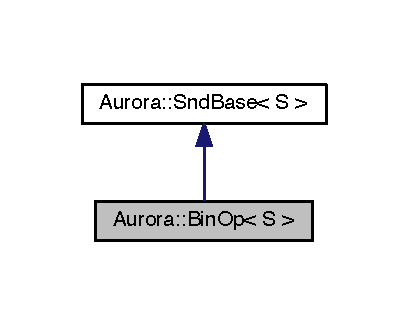
\includegraphics[width=196pt]{class_aurora_1_1_bin_op__inherit__graph}
\end{center}
\end{figure}


Collaboration diagram for Aurora\+:\+:Bin\+Op$<$ S $>$\+:\nopagebreak
\begin{figure}[H]
\begin{center}
\leavevmode
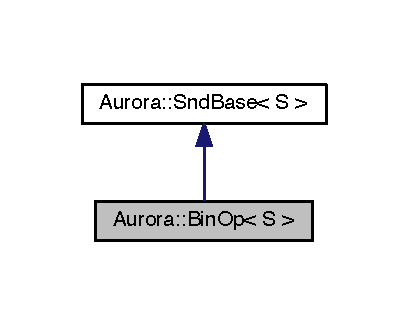
\includegraphics[width=196pt]{class_aurora_1_1_bin_op__coll__graph}
\end{center}
\end{figure}
\subsection*{Public Member Functions}
\begin{DoxyCompactItemize}
\item 
\hyperlink{class_aurora_1_1_bin_op_aa8b5c6b77e89f4c73847716a695be047}{Bin\+Op} (const std\+::function$<$ S(S, S)$>$ \&f, std\+::size\+\_\+t \hyperlink{class_aurora_1_1_snd_base_af9e21aaf411b17f7a8221c991ce5d291}{vsize}=\hyperlink{namespace_aurora_afaaddf667a06e7ce23c667a8b7295263}{def\+\_\+vsize})
\item 
const std\+::vector$<$ S $>$ \& \hyperlink{class_aurora_1_1_bin_op_aef7a0a9a5daa40c22e540f08ca928fab}{operator()} (S a, const std\+::vector$<$ S $>$ \&s)
\item 
const std\+::vector$<$ S $>$ \& \hyperlink{class_aurora_1_1_bin_op_a488095df0eb9f16da6643476dec9e51c}{operator()} (const std\+::vector$<$ S $>$ \&s, S a)
\item 
const std\+::vector$<$ S $>$ \& \hyperlink{class_aurora_1_1_bin_op_abe8a0b7666caeda012d9ac18f889e116}{operator()} (const std\+::vector$<$ S $>$ \&s1, const std\+::vector$<$ S $>$ \&s2)
\item 
void \hyperlink{class_aurora_1_1_bin_op_aa440ae97cd1e9f0e1aaa077a57850f3d}{func} (const std\+::function$<$ S(S, S)$>$ \&f)
\end{DoxyCompactItemize}
\subsection*{Additional Inherited Members}


\subsection{Detailed Description}
\subsubsection*{template$<$typename S$>$\newline
class Aurora\+::\+Bin\+Op$<$ S $>$}

\hyperlink{class_aurora_1_1_bin_op}{Bin\+Op} class ~\newline
Binary operations ~\newline
S\+: sample type 

\subsection{Constructor \& Destructor Documentation}
\mbox{\Hypertarget{class_aurora_1_1_bin_op_aa8b5c6b77e89f4c73847716a695be047}\label{class_aurora_1_1_bin_op_aa8b5c6b77e89f4c73847716a695be047}} 
\index{Aurora\+::\+Bin\+Op@{Aurora\+::\+Bin\+Op}!Bin\+Op@{Bin\+Op}}
\index{Bin\+Op@{Bin\+Op}!Aurora\+::\+Bin\+Op@{Aurora\+::\+Bin\+Op}}
\subsubsection{\texorpdfstring{Bin\+Op()}{BinOp()}}
{\footnotesize\ttfamily template$<$typename S $>$ \\
\hyperlink{class_aurora_1_1_bin_op}{Aurora\+::\+Bin\+Op}$<$ S $>$\+::\hyperlink{class_aurora_1_1_bin_op}{Bin\+Op} (\begin{DoxyParamCaption}\item[{const std\+::function$<$ S(S, S)$>$ \&}]{f,  }\item[{std\+::size\+\_\+t}]{vsize = {\ttfamily \hyperlink{namespace_aurora_afaaddf667a06e7ce23c667a8b7295263}{def\+\_\+vsize}} }\end{DoxyParamCaption})\hspace{0.3cm}{\ttfamily [inline]}}

Constructor ~\newline
f\+: binary operation function ~\newline
vsize\+: signal vector size 

\subsection{Member Function Documentation}
\mbox{\Hypertarget{class_aurora_1_1_bin_op_aa440ae97cd1e9f0e1aaa077a57850f3d}\label{class_aurora_1_1_bin_op_aa440ae97cd1e9f0e1aaa077a57850f3d}} 
\index{Aurora\+::\+Bin\+Op@{Aurora\+::\+Bin\+Op}!func@{func}}
\index{func@{func}!Aurora\+::\+Bin\+Op@{Aurora\+::\+Bin\+Op}}
\subsubsection{\texorpdfstring{func()}{func()}}
{\footnotesize\ttfamily template$<$typename S $>$ \\
void \hyperlink{class_aurora_1_1_bin_op}{Aurora\+::\+Bin\+Op}$<$ S $>$\+::func (\begin{DoxyParamCaption}\item[{const std\+::function$<$ S(S, S)$>$ \&}]{f }\end{DoxyParamCaption})\hspace{0.3cm}{\ttfamily [inline]}}

set the operator function ~\newline
f\+: binary operator function to be used \mbox{\Hypertarget{class_aurora_1_1_bin_op_aef7a0a9a5daa40c22e540f08ca928fab}\label{class_aurora_1_1_bin_op_aef7a0a9a5daa40c22e540f08ca928fab}} 
\index{Aurora\+::\+Bin\+Op@{Aurora\+::\+Bin\+Op}!operator()@{operator()}}
\index{operator()@{operator()}!Aurora\+::\+Bin\+Op@{Aurora\+::\+Bin\+Op}}
\subsubsection{\texorpdfstring{operator()()}{operator()()}\hspace{0.1cm}{\footnotesize\ttfamily [1/3]}}
{\footnotesize\ttfamily template$<$typename S $>$ \\
const std\+::vector$<$S$>$\& \hyperlink{class_aurora_1_1_bin_op}{Aurora\+::\+Bin\+Op}$<$ S $>$\+::operator() (\begin{DoxyParamCaption}\item[{S}]{a,  }\item[{const std\+::vector$<$ S $>$ \&}]{s }\end{DoxyParamCaption})\hspace{0.3cm}{\ttfamily [inline]}}

Binary operation ~\newline
a\+: scalar input ~\newline
s\+: signal input ~\newline
returns reference to object signal vector \mbox{\Hypertarget{class_aurora_1_1_bin_op_a488095df0eb9f16da6643476dec9e51c}\label{class_aurora_1_1_bin_op_a488095df0eb9f16da6643476dec9e51c}} 
\index{Aurora\+::\+Bin\+Op@{Aurora\+::\+Bin\+Op}!operator()@{operator()}}
\index{operator()@{operator()}!Aurora\+::\+Bin\+Op@{Aurora\+::\+Bin\+Op}}
\subsubsection{\texorpdfstring{operator()()}{operator()()}\hspace{0.1cm}{\footnotesize\ttfamily [2/3]}}
{\footnotesize\ttfamily template$<$typename S $>$ \\
const std\+::vector$<$S$>$\& \hyperlink{class_aurora_1_1_bin_op}{Aurora\+::\+Bin\+Op}$<$ S $>$\+::operator() (\begin{DoxyParamCaption}\item[{const std\+::vector$<$ S $>$ \&}]{s,  }\item[{S}]{a }\end{DoxyParamCaption})\hspace{0.3cm}{\ttfamily [inline]}}

Binary operation ~\newline
s\+: signal input ~\newline
a\+: scalar input ~\newline
returns reference to object signal vector \mbox{\Hypertarget{class_aurora_1_1_bin_op_abe8a0b7666caeda012d9ac18f889e116}\label{class_aurora_1_1_bin_op_abe8a0b7666caeda012d9ac18f889e116}} 
\index{Aurora\+::\+Bin\+Op@{Aurora\+::\+Bin\+Op}!operator()@{operator()}}
\index{operator()@{operator()}!Aurora\+::\+Bin\+Op@{Aurora\+::\+Bin\+Op}}
\subsubsection{\texorpdfstring{operator()()}{operator()()}\hspace{0.1cm}{\footnotesize\ttfamily [3/3]}}
{\footnotesize\ttfamily template$<$typename S $>$ \\
const std\+::vector$<$S$>$\& \hyperlink{class_aurora_1_1_bin_op}{Aurora\+::\+Bin\+Op}$<$ S $>$\+::operator() (\begin{DoxyParamCaption}\item[{const std\+::vector$<$ S $>$ \&}]{s1,  }\item[{const std\+::vector$<$ S $>$ \&}]{s2 }\end{DoxyParamCaption})\hspace{0.3cm}{\ttfamily [inline]}}

Binary operation ~\newline
s1\+: signal input 1 ~\newline
s2\+: signal input 2 ~\newline
returns reference to object signal vector 

The documentation for this class was generated from the following file\+:\begin{DoxyCompactItemize}
\item 
\hyperlink{_snd_base_8h}{Snd\+Base.\+h}\end{DoxyCompactItemize}

\hypertarget{class_aurora_1_1_bl_osc}{}\section{Aurora\+:\+:Bl\+Osc$<$ S, FN $>$ Class Template Reference}
\label{class_aurora_1_1_bl_osc}\index{Aurora\+::\+Bl\+Osc$<$ S, F\+N $>$@{Aurora\+::\+Bl\+Osc$<$ S, F\+N $>$}}


{\ttfamily \#include $<$Bl\+Osc.\+h$>$}



Inheritance diagram for Aurora\+:\+:Bl\+Osc$<$ S, FN $>$\+:
\nopagebreak
\begin{figure}[H]
\begin{center}
\leavevmode
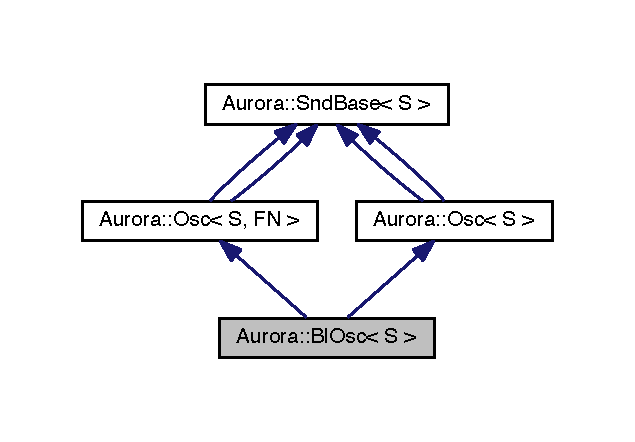
\includegraphics[width=202pt]{class_aurora_1_1_bl_osc__inherit__graph}
\end{center}
\end{figure}


Collaboration diagram for Aurora\+:\+:Bl\+Osc$<$ S, FN $>$\+:
\nopagebreak
\begin{figure}[H]
\begin{center}
\leavevmode
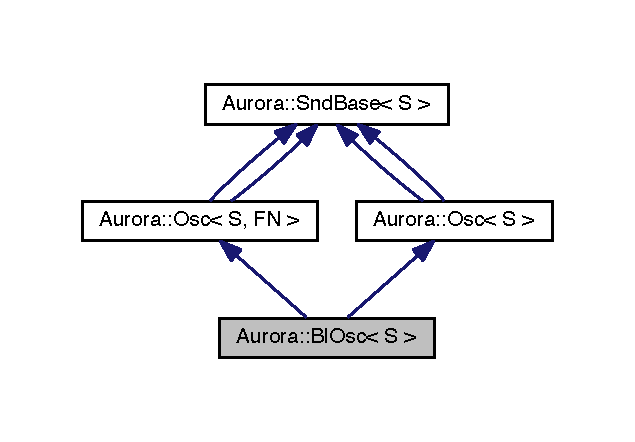
\includegraphics[width=202pt]{class_aurora_1_1_bl_osc__coll__graph}
\end{center}
\end{figure}
\subsection*{Public Member Functions}
\begin{DoxyCompactItemize}
\item 
\hyperlink{class_aurora_1_1_bl_osc_a70a21ed3ae7e69c236b9af7e64911920}{Bl\+Osc} (const \hyperlink{class_aurora_1_1_table_set}{Table\+Set}$<$ S $>$ $\ast$t, S \hyperlink{class_aurora_1_1_osc_a10d968f92bf489112dd990c15cda6780}{fs}=(S) \hyperlink{namespace_aurora_ad49263d809bea98dd422e95bc91bc03e}{def\+\_\+sr}, std\+::size\+\_\+t \hyperlink{class_aurora_1_1_snd_base_af9e21aaf411b17f7a8221c991ce5d291}{vsize}=\hyperlink{namespace_aurora_afaaddf667a06e7ce23c667a8b7295263}{def\+\_\+vsize})
\item 
void \hyperlink{class_aurora_1_1_bl_osc_a053c6740b4b419c6c03e246188906ebc}{waveset} (const \hyperlink{class_aurora_1_1_table_set}{Table\+Set}$<$ S $>$ $\ast$t)
\end{DoxyCompactItemize}


\subsection{Detailed Description}
\subsubsection*{template$<$typename S, S($\ast$)(double, const std\+::vector$<$ S $>$ $\ast$) FN = lookupi$<$\+S$>$$>$\newline
class Aurora\+::\+Bl\+Osc$<$ S, F\+N $>$}

\hyperlink{class_aurora_1_1_bl_osc}{Bl\+Osc} class ~\newline
Bandlimited wavetable oscillator. ~\newline
S\+: sample type ~\newline
FN\+: oscillator function 

\subsection{Constructor \& Destructor Documentation}
\mbox{\Hypertarget{class_aurora_1_1_bl_osc_a70a21ed3ae7e69c236b9af7e64911920}\label{class_aurora_1_1_bl_osc_a70a21ed3ae7e69c236b9af7e64911920}} 
\index{Aurora\+::\+Bl\+Osc@{Aurora\+::\+Bl\+Osc}!Bl\+Osc@{Bl\+Osc}}
\index{Bl\+Osc@{Bl\+Osc}!Aurora\+::\+Bl\+Osc@{Aurora\+::\+Bl\+Osc}}
\subsubsection{\texorpdfstring{Bl\+Osc()}{BlOsc()}}
{\footnotesize\ttfamily template$<$typename S , S($\ast$)(double, const std\+::vector$<$ S $>$ $\ast$) FN = lookupi$<$\+S$>$$>$ \\
\hyperlink{class_aurora_1_1_bl_osc}{Aurora\+::\+Bl\+Osc}$<$ S, FN $>$\+::\hyperlink{class_aurora_1_1_bl_osc}{Bl\+Osc} (\begin{DoxyParamCaption}\item[{const \hyperlink{class_aurora_1_1_table_set}{Table\+Set}$<$ S $>$ $\ast$}]{t,  }\item[{S}]{fs = {\ttfamily (S)\hyperlink{namespace_aurora_ad49263d809bea98dd422e95bc91bc03e}{def\+\_\+sr}},  }\item[{std\+::size\+\_\+t}]{vsize = {\ttfamily \hyperlink{namespace_aurora_afaaddf667a06e7ce23c667a8b7295263}{def\+\_\+vsize}} }\end{DoxyParamCaption})\hspace{0.3cm}{\ttfamily [inline]}}

Constructor ~\newline
t\+: wavetable set ~\newline
fs\+: sampling rate ~\newline
vsize\+: vector size 

\subsection{Member Function Documentation}
\mbox{\Hypertarget{class_aurora_1_1_bl_osc_a053c6740b4b419c6c03e246188906ebc}\label{class_aurora_1_1_bl_osc_a053c6740b4b419c6c03e246188906ebc}} 
\index{Aurora\+::\+Bl\+Osc@{Aurora\+::\+Bl\+Osc}!waveset@{waveset}}
\index{waveset@{waveset}!Aurora\+::\+Bl\+Osc@{Aurora\+::\+Bl\+Osc}}
\subsubsection{\texorpdfstring{waveset()}{waveset()}}
{\footnotesize\ttfamily template$<$typename S , S($\ast$)(double, const std\+::vector$<$ S $>$ $\ast$) FN = lookupi$<$\+S$>$$>$ \\
void \hyperlink{class_aurora_1_1_bl_osc}{Aurora\+::\+Bl\+Osc}$<$ S, FN $>$\+::waveset (\begin{DoxyParamCaption}\item[{const \hyperlink{class_aurora_1_1_table_set}{Table\+Set}$<$ S $>$ $\ast$}]{t }\end{DoxyParamCaption})\hspace{0.3cm}{\ttfamily [inline]}}

Change the wavetable set t\+: wavetable set 

The documentation for this class was generated from the following file\+:\begin{DoxyCompactItemize}
\item 
\hyperlink{_bl_osc_8h}{Bl\+Osc.\+h}\end{DoxyCompactItemize}

\hypertarget{class_aurora_1_1_env}{}\doxysection{Aurora\+::Env\texorpdfstring{$<$}{<} S, FN \texorpdfstring{$>$}{>} Class Template Reference}
\label{class_aurora_1_1_env}\index{Aurora::Env$<$ S, FN $>$@{Aurora::Env$<$ S, FN $>$}}


{\ttfamily \#include $<$Env.\+h$>$}



Inheritance diagram for Aurora\+::Env\texorpdfstring{$<$}{<} S, FN \texorpdfstring{$>$}{>}\+:
% FIG 0


Collaboration diagram for Aurora\+::Env\texorpdfstring{$<$}{<} S, FN \texorpdfstring{$>$}{>}\+:
% FIG 1
\doxysubsection*{Public Member Functions}
\begin{DoxyCompactItemize}
\item 
\mbox{\hyperlink{class_aurora_1_1_env_a500fe7e05d736a21c801ffa480aceed7}{Env}} (std\+::function$<$ S(double, S, S)$>$ f, S rt, S \mbox{\hyperlink{class_aurora_1_1_env_a8b83ca686cce4fc31b03b1de847bc062}{fs}}=\mbox{\hyperlink{namespace_aurora_ad49263d809bea98dd422e95bc91bc03e}{def\+\_\+sr}}, std\+::size\+\_\+t \mbox{\hyperlink{class_aurora_1_1_snd_base_af9e21aaf411b17f7a8221c991ce5d291}{vsize}}=\mbox{\hyperlink{namespace_aurora_afaaddf667a06e7ce23c667a8b7295263}{def\+\_\+vsize}})
\item 
\mbox{\hyperlink{class_aurora_1_1_env_a3ea4ee867e90f80331819cceacc55942}{Env}} (S \&a, S \&b, S \&c, S rt, S \mbox{\hyperlink{class_aurora_1_1_env_a8b83ca686cce4fc31b03b1de847bc062}{fs}}=\mbox{\hyperlink{namespace_aurora_ad49263d809bea98dd422e95bc91bc03e}{def\+\_\+sr}}, std\+::size\+\_\+t \mbox{\hyperlink{class_aurora_1_1_snd_base_af9e21aaf411b17f7a8221c991ce5d291}{vsize}}=\mbox{\hyperlink{namespace_aurora_afaaddf667a06e7ce23c667a8b7295263}{def\+\_\+vsize}})
\item 
void \mbox{\hyperlink{class_aurora_1_1_env_a65103efd17db785d902c32260ab79908}{release}} (S t)
\item 
S \mbox{\hyperlink{class_aurora_1_1_env_aafec7ceda90a9a8c91c7b7feef56ddf1}{release}} ()
\item 
void \mbox{\hyperlink{class_aurora_1_1_env_a87a6a75c7470021f42c412ecfbe9fab4}{retrigger}} ()
\item 
const std\+::vector$<$ S $>$ \& \mbox{\hyperlink{class_aurora_1_1_env_a26aa8e7e6fc71eadda232af5c1c5b960}{operator()}} (bool gate)
\item 
const std\+::vector$<$ S $>$ \& \mbox{\hyperlink{class_aurora_1_1_env_a4471a8c3abcf677c2e31aa0e214c529b}{operator()}} (S offs, S scal, bool gate)
\item 
const std\+::vector$<$ S $>$ \& \mbox{\hyperlink{class_aurora_1_1_env_ad87b147f31ac28655e61a8dac0ca442b}{operator()}} (const std\+::vector$<$ S $>$ \&in, bool gate)
\item 
S \mbox{\hyperlink{class_aurora_1_1_env_a8b83ca686cce4fc31b03b1de847bc062}{fs}} () const
\item 
void \mbox{\hyperlink{class_aurora_1_1_env_a12db5d285b749a7e1fed988d344d3bc9}{reset}} (S \mbox{\hyperlink{class_aurora_1_1_env_a8b83ca686cce4fc31b03b1de847bc062}{fs}})
\item 
void \mbox{\hyperlink{class_aurora_1_1_env_a92aec91bb78127cf50d5d841870cce14}{func}} (const std\+::function$<$ S(double, S, S)$>$ f)
\end{DoxyCompactItemize}


\doxysubsection{Detailed Description}
\subsubsection*{template$<$typename S, S($\ast$)(S, S, S, double, S, S) FN = ads$>$\newline
class Aurora\+::\+Env$<$ S, FN $>$}
\mbox{\hyperlink{class_aurora_1_1_env}{Env}} class ~\newline
Generic envelope ~\newline
S\+: sample type ~\newline
FN\+: envelope function 

\doxysubsection{Constructor \& Destructor Documentation}
\mbox{\Hypertarget{class_aurora_1_1_env_a500fe7e05d736a21c801ffa480aceed7}\label{class_aurora_1_1_env_a500fe7e05d736a21c801ffa480aceed7}} 
\index{Aurora::Env$<$ S, FN $>$@{Aurora::Env$<$ S, FN $>$}!Env@{Env}}
\index{Env@{Env}!Aurora::Env$<$ S, FN $>$@{Aurora::Env$<$ S, FN $>$}}
\doxysubsubsection{\texorpdfstring{Env()}{Env()}\hspace{0.1cm}{\footnotesize\ttfamily [1/2]}}
{\footnotesize\ttfamily template$<$typename S , S($\ast$)(S, S, S, double, S, S) FN = ads$>$ \\
\mbox{\hyperlink{class_aurora_1_1_env}{Aurora\+::\+Env}}$<$ S, FN $>$\+::\+Env (\begin{DoxyParamCaption}\item[{std\+::function$<$ S(double, S, S)$>$}]{f,  }\item[{S}]{rt,  }\item[{S}]{fs = {\ttfamily \mbox{\hyperlink{namespace_aurora_ad49263d809bea98dd422e95bc91bc03e}{def\+\_\+sr}}},  }\item[{std\+::size\+\_\+t}]{vsize = {\ttfamily \mbox{\hyperlink{namespace_aurora_afaaddf667a06e7ce23c667a8b7295263}{def\+\_\+vsize}}} }\end{DoxyParamCaption})\hspace{0.3cm}{\ttfamily [inline]}}

Constructor ~\newline
f\+: envelope function ~\newline
rt\+: release time ~\newline
fs\+: sampling rate ~\newline
vsize\+: signal vector size \mbox{\Hypertarget{class_aurora_1_1_env_a3ea4ee867e90f80331819cceacc55942}\label{class_aurora_1_1_env_a3ea4ee867e90f80331819cceacc55942}} 
\index{Aurora::Env$<$ S, FN $>$@{Aurora::Env$<$ S, FN $>$}!Env@{Env}}
\index{Env@{Env}!Aurora::Env$<$ S, FN $>$@{Aurora::Env$<$ S, FN $>$}}
\doxysubsubsection{\texorpdfstring{Env()}{Env()}\hspace{0.1cm}{\footnotesize\ttfamily [2/2]}}
{\footnotesize\ttfamily template$<$typename S , S($\ast$)(S, S, S, double, S, S) FN = ads$>$ \\
\mbox{\hyperlink{class_aurora_1_1_env}{Aurora\+::\+Env}}$<$ S, FN $>$\+::\+Env (\begin{DoxyParamCaption}\item[{S \&}]{a,  }\item[{S \&}]{b,  }\item[{S \&}]{c,  }\item[{S}]{rt,  }\item[{S}]{fs = {\ttfamily \mbox{\hyperlink{namespace_aurora_ad49263d809bea98dd422e95bc91bc03e}{def\+\_\+sr}}},  }\item[{std\+::size\+\_\+t}]{vsize = {\ttfamily \mbox{\hyperlink{namespace_aurora_afaaddf667a06e7ce23c667a8b7295263}{def\+\_\+vsize}}} }\end{DoxyParamCaption})\hspace{0.3cm}{\ttfamily [inline]}}

Constructor ~\newline
a\+: env fn parameter 1 ~\newline
b\+: env fn parameter 2 ~\newline
c\+: env fn parameter 3~\newline
rt\+: release time ~\newline
fs\+: sampling rate ~\newline
vsize\+: signal vector size 

\doxysubsection{Member Function Documentation}
\mbox{\Hypertarget{class_aurora_1_1_env_a8b83ca686cce4fc31b03b1de847bc062}\label{class_aurora_1_1_env_a8b83ca686cce4fc31b03b1de847bc062}} 
\index{Aurora::Env$<$ S, FN $>$@{Aurora::Env$<$ S, FN $>$}!fs@{fs}}
\index{fs@{fs}!Aurora::Env$<$ S, FN $>$@{Aurora::Env$<$ S, FN $>$}}
\doxysubsubsection{\texorpdfstring{fs()}{fs()}}
{\footnotesize\ttfamily template$<$typename S , S($\ast$)(S, S, S, double, S, S) FN = ads$>$ \\
S \mbox{\hyperlink{class_aurora_1_1_env}{Aurora\+::\+Env}}$<$ S, FN $>$\+::fs (\begin{DoxyParamCaption}{ }\end{DoxyParamCaption}) const\hspace{0.3cm}{\ttfamily [inline]}}

Sampling rate query ~\newline
returns sampling rate \mbox{\Hypertarget{class_aurora_1_1_env_a92aec91bb78127cf50d5d841870cce14}\label{class_aurora_1_1_env_a92aec91bb78127cf50d5d841870cce14}} 
\index{Aurora::Env$<$ S, FN $>$@{Aurora::Env$<$ S, FN $>$}!func@{func}}
\index{func@{func}!Aurora::Env$<$ S, FN $>$@{Aurora::Env$<$ S, FN $>$}}
\doxysubsubsection{\texorpdfstring{func()}{func()}}
{\footnotesize\ttfamily template$<$typename S , S($\ast$)(S, S, S, double, S, S) FN = ads$>$ \\
void \mbox{\hyperlink{class_aurora_1_1_env}{Aurora\+::\+Env}}$<$ S, FN $>$\+::func (\begin{DoxyParamCaption}\item[{const std\+::function$<$ S(double, S, S)$>$}]{f }\end{DoxyParamCaption})\hspace{0.3cm}{\ttfamily [inline]}}

set the envelope function ~\newline
f\+: envelope function to be used \mbox{\Hypertarget{class_aurora_1_1_env_a26aa8e7e6fc71eadda232af5c1c5b960}\label{class_aurora_1_1_env_a26aa8e7e6fc71eadda232af5c1c5b960}} 
\index{Aurora::Env$<$ S, FN $>$@{Aurora::Env$<$ S, FN $>$}!operator()@{operator()}}
\index{operator()@{operator()}!Aurora::Env$<$ S, FN $>$@{Aurora::Env$<$ S, FN $>$}}
\doxysubsubsection{\texorpdfstring{operator()()}{operator()()}\hspace{0.1cm}{\footnotesize\ttfamily [1/3]}}
{\footnotesize\ttfamily template$<$typename S , S($\ast$)(S, S, S, double, S, S) FN = ads$>$ \\
const std\+::vector$<$ S $>$ \& \mbox{\hyperlink{class_aurora_1_1_env}{Aurora\+::\+Env}}$<$ S, FN $>$\+::operator() (\begin{DoxyParamCaption}\item[{bool}]{gate }\end{DoxyParamCaption})\hspace{0.3cm}{\ttfamily [inline]}}

Envelope ~\newline
gate\+: envelope gate \mbox{\Hypertarget{class_aurora_1_1_env_ad87b147f31ac28655e61a8dac0ca442b}\label{class_aurora_1_1_env_ad87b147f31ac28655e61a8dac0ca442b}} 
\index{Aurora::Env$<$ S, FN $>$@{Aurora::Env$<$ S, FN $>$}!operator()@{operator()}}
\index{operator()@{operator()}!Aurora::Env$<$ S, FN $>$@{Aurora::Env$<$ S, FN $>$}}
\doxysubsubsection{\texorpdfstring{operator()()}{operator()()}\hspace{0.1cm}{\footnotesize\ttfamily [2/3]}}
{\footnotesize\ttfamily template$<$typename S , S($\ast$)(S, S, S, double, S, S) FN = ads$>$ \\
const std\+::vector$<$ S $>$ \& \mbox{\hyperlink{class_aurora_1_1_env}{Aurora\+::\+Env}}$<$ S, FN $>$\+::operator() (\begin{DoxyParamCaption}\item[{const std\+::vector$<$ S $>$ \&}]{in,  }\item[{bool}]{gate }\end{DoxyParamCaption})\hspace{0.3cm}{\ttfamily [inline]}}

Envelope ~\newline
in\+: input signal gate\+: envelope gate \mbox{\Hypertarget{class_aurora_1_1_env_a4471a8c3abcf677c2e31aa0e214c529b}\label{class_aurora_1_1_env_a4471a8c3abcf677c2e31aa0e214c529b}} 
\index{Aurora::Env$<$ S, FN $>$@{Aurora::Env$<$ S, FN $>$}!operator()@{operator()}}
\index{operator()@{operator()}!Aurora::Env$<$ S, FN $>$@{Aurora::Env$<$ S, FN $>$}}
\doxysubsubsection{\texorpdfstring{operator()()}{operator()()}\hspace{0.1cm}{\footnotesize\ttfamily [3/3]}}
{\footnotesize\ttfamily template$<$typename S , S($\ast$)(S, S, S, double, S, S) FN = ads$>$ \\
const std\+::vector$<$ S $>$ \& \mbox{\hyperlink{class_aurora_1_1_env}{Aurora\+::\+Env}}$<$ S, FN $>$\+::operator() (\begin{DoxyParamCaption}\item[{S}]{offs,  }\item[{S}]{scal,  }\item[{bool}]{gate }\end{DoxyParamCaption})\hspace{0.3cm}{\ttfamily [inline]}}

Envelope ~\newline
offs\+: sig offset scal\+: sig scale gate\+: envelope gate \mbox{\Hypertarget{class_aurora_1_1_env_aafec7ceda90a9a8c91c7b7feef56ddf1}\label{class_aurora_1_1_env_aafec7ceda90a9a8c91c7b7feef56ddf1}} 
\index{Aurora::Env$<$ S, FN $>$@{Aurora::Env$<$ S, FN $>$}!release@{release}}
\index{release@{release}!Aurora::Env$<$ S, FN $>$@{Aurora::Env$<$ S, FN $>$}}
\doxysubsubsection{\texorpdfstring{release()}{release()}\hspace{0.1cm}{\footnotesize\ttfamily [1/2]}}
{\footnotesize\ttfamily template$<$typename S , S($\ast$)(S, S, S, double, S, S) FN = ads$>$ \\
S \mbox{\hyperlink{class_aurora_1_1_env}{Aurora\+::\+Env}}$<$ S, FN $>$\+::release (\begin{DoxyParamCaption}{ }\end{DoxyParamCaption})\hspace{0.3cm}{\ttfamily [inline]}}

\mbox{\Hypertarget{class_aurora_1_1_env_a65103efd17db785d902c32260ab79908}\label{class_aurora_1_1_env_a65103efd17db785d902c32260ab79908}} 
\index{Aurora::Env$<$ S, FN $>$@{Aurora::Env$<$ S, FN $>$}!release@{release}}
\index{release@{release}!Aurora::Env$<$ S, FN $>$@{Aurora::Env$<$ S, FN $>$}}
\doxysubsubsection{\texorpdfstring{release()}{release()}\hspace{0.1cm}{\footnotesize\ttfamily [2/2]}}
{\footnotesize\ttfamily template$<$typename S , S($\ast$)(S, S, S, double, S, S) FN = ads$>$ \\
void \mbox{\hyperlink{class_aurora_1_1_env}{Aurora\+::\+Env}}$<$ S, FN $>$\+::release (\begin{DoxyParamCaption}\item[{S}]{t }\end{DoxyParamCaption})\hspace{0.3cm}{\ttfamily [inline]}}

Release time setter rt\+: release time \mbox{\Hypertarget{class_aurora_1_1_env_a12db5d285b749a7e1fed988d344d3bc9}\label{class_aurora_1_1_env_a12db5d285b749a7e1fed988d344d3bc9}} 
\index{Aurora::Env$<$ S, FN $>$@{Aurora::Env$<$ S, FN $>$}!reset@{reset}}
\index{reset@{reset}!Aurora::Env$<$ S, FN $>$@{Aurora::Env$<$ S, FN $>$}}
\doxysubsubsection{\texorpdfstring{reset()}{reset()}}
{\footnotesize\ttfamily template$<$typename S , S($\ast$)(S, S, S, double, S, S) FN = ads$>$ \\
void \mbox{\hyperlink{class_aurora_1_1_env}{Aurora\+::\+Env}}$<$ S, FN $>$\+::reset (\begin{DoxyParamCaption}\item[{S}]{fs }\end{DoxyParamCaption})\hspace{0.3cm}{\ttfamily [inline]}}

reset the envelope ~\newline
fs\+: sampling rate \mbox{\Hypertarget{class_aurora_1_1_env_a87a6a75c7470021f42c412ecfbe9fab4}\label{class_aurora_1_1_env_a87a6a75c7470021f42c412ecfbe9fab4}} 
\index{Aurora::Env$<$ S, FN $>$@{Aurora::Env$<$ S, FN $>$}!retrigger@{retrigger}}
\index{retrigger@{retrigger}!Aurora::Env$<$ S, FN $>$@{Aurora::Env$<$ S, FN $>$}}
\doxysubsubsection{\texorpdfstring{retrigger()}{retrigger()}}
{\footnotesize\ttfamily template$<$typename S , S($\ast$)(S, S, S, double, S, S) FN = ads$>$ \\
void \mbox{\hyperlink{class_aurora_1_1_env}{Aurora\+::\+Env}}$<$ S, FN $>$\+::retrigger (\begin{DoxyParamCaption}{ }\end{DoxyParamCaption})\hspace{0.3cm}{\ttfamily [inline]}}

Retrigger 

The documentation for this class was generated from the following file\+:\begin{DoxyCompactItemize}
\item 
\mbox{\hyperlink{_env_8h}{Env.\+h}}\end{DoxyCompactItemize}

\hypertarget{class_aurora_1_1_f_f_t}{}\section{Aurora\+:\+:F\+FT$<$ S $>$ Class Template Reference}
\label{class_aurora_1_1_f_f_t}\index{Aurora\+::\+F\+F\+T$<$ S $>$@{Aurora\+::\+F\+F\+T$<$ S $>$}}


{\ttfamily \#include $<$F\+F\+T.\+h$>$}

\subsection*{Public Member Functions}
\begin{DoxyCompactItemize}
\item 
\hyperlink{class_aurora_1_1_f_f_t_ab98366f22f4fde5a1b0e32445eedcf3c}{F\+FT} (std\+::size\+\_\+t N, bool packed=true)
\item 
std\+::size\+\_\+t \hyperlink{class_aurora_1_1_f_f_t_ad0149c60672d3f4e64850dde22f5b163}{size} ()
\item 
void \hyperlink{class_aurora_1_1_f_f_t_a8325de64c8b9f208ed0bc8db3f74e4c7}{transform} (std\+::vector$<$ std\+::complex$<$ S $>$$>$ \&s, bool dir)
\item 
const std\+::complex$<$ S $>$ $\ast$ \hyperlink{class_aurora_1_1_f_f_t_a51ed1e25953c12b7f4cc145d19ee5cd8}{transform} (const std\+::vector$<$ S $>$ \&r)
\item 
const S $\ast$ \hyperlink{class_aurora_1_1_f_f_t_aa0912d8abdeb15ff84d82a5cc59cb150}{transform} (const std\+::vector$<$ std\+::complex$<$ S $>$$>$ \&sp, bool pckd=true)
\end{DoxyCompactItemize}


\subsection{Detailed Description}
\subsubsection*{template$<$typename S$>$\newline
class Aurora\+::\+F\+F\+T$<$ S $>$}

\hyperlink{class_aurora_1_1_f_f_t}{F\+FT} class ~\newline
Radix-\/2 fast Fourier transform ~\newline
S\+: sample type 

\subsection{Constructor \& Destructor Documentation}
\mbox{\Hypertarget{class_aurora_1_1_f_f_t_ab98366f22f4fde5a1b0e32445eedcf3c}\label{class_aurora_1_1_f_f_t_ab98366f22f4fde5a1b0e32445eedcf3c}} 
\index{Aurora\+::\+F\+FT@{Aurora\+::\+F\+FT}!F\+FT@{F\+FT}}
\index{F\+FT@{F\+FT}!Aurora\+::\+F\+FT@{Aurora\+::\+F\+FT}}
\subsubsection{\texorpdfstring{F\+F\+T()}{FFT()}}
{\footnotesize\ttfamily template$<$typename S$>$ \\
\hyperlink{class_aurora_1_1_f_f_t}{Aurora\+::\+F\+FT}$<$ S $>$\+::\hyperlink{class_aurora_1_1_f_f_t}{F\+FT} (\begin{DoxyParamCaption}\item[{std\+::size\+\_\+t}]{N,  }\item[{bool}]{packed = {\ttfamily true} }\end{DoxyParamCaption})\hspace{0.3cm}{\ttfamily [inline]}}

Constructor ~\newline
N\+: transform size ~\newline
packed\+: complex data format in packed form (true) or not 

\subsection{Member Function Documentation}
\mbox{\Hypertarget{class_aurora_1_1_f_f_t_ad0149c60672d3f4e64850dde22f5b163}\label{class_aurora_1_1_f_f_t_ad0149c60672d3f4e64850dde22f5b163}} 
\index{Aurora\+::\+F\+FT@{Aurora\+::\+F\+FT}!size@{size}}
\index{size@{size}!Aurora\+::\+F\+FT@{Aurora\+::\+F\+FT}}
\subsubsection{\texorpdfstring{size()}{size()}}
{\footnotesize\ttfamily template$<$typename S$>$ \\
std\+::size\+\_\+t \hyperlink{class_aurora_1_1_f_f_t}{Aurora\+::\+F\+FT}$<$ S $>$\+::size (\begin{DoxyParamCaption}{ }\end{DoxyParamCaption})\hspace{0.3cm}{\ttfamily [inline]}}

\mbox{\Hypertarget{class_aurora_1_1_f_f_t_a8325de64c8b9f208ed0bc8db3f74e4c7}\label{class_aurora_1_1_f_f_t_a8325de64c8b9f208ed0bc8db3f74e4c7}} 
\index{Aurora\+::\+F\+FT@{Aurora\+::\+F\+FT}!transform@{transform}}
\index{transform@{transform}!Aurora\+::\+F\+FT@{Aurora\+::\+F\+FT}}
\subsubsection{\texorpdfstring{transform()}{transform()}\hspace{0.1cm}{\footnotesize\ttfamily [1/3]}}
{\footnotesize\ttfamily template$<$typename S$>$ \\
void \hyperlink{class_aurora_1_1_f_f_t}{Aurora\+::\+F\+FT}$<$ S $>$\+::transform (\begin{DoxyParamCaption}\item[{std\+::vector$<$ std\+::complex$<$ S $>$$>$ \&}]{s,  }\item[{bool}]{dir }\end{DoxyParamCaption})\hspace{0.3cm}{\ttfamily [inline]}}

In-\/place complex-\/to-\/complex \hyperlink{class_aurora_1_1_f_f_t}{F\+FT} ~\newline
data\+: data to be transformed ~\newline
dir\+: true for forward operation, false for inverse ~\newline
pckd\+: true for packed data (first point is DC,Nyq) Size of data is expected to be a power-\/of-\/two. \mbox{\Hypertarget{class_aurora_1_1_f_f_t_a51ed1e25953c12b7f4cc145d19ee5cd8}\label{class_aurora_1_1_f_f_t_a51ed1e25953c12b7f4cc145d19ee5cd8}} 
\index{Aurora\+::\+F\+FT@{Aurora\+::\+F\+FT}!transform@{transform}}
\index{transform@{transform}!Aurora\+::\+F\+FT@{Aurora\+::\+F\+FT}}
\subsubsection{\texorpdfstring{transform()}{transform()}\hspace{0.1cm}{\footnotesize\ttfamily [2/3]}}
{\footnotesize\ttfamily template$<$typename S$>$ \\
const std\+::complex$<$S$>$$\ast$ \hyperlink{class_aurora_1_1_f_f_t}{Aurora\+::\+F\+FT}$<$ S $>$\+::transform (\begin{DoxyParamCaption}\item[{const std\+::vector$<$ S $>$ \&}]{r }\end{DoxyParamCaption})\hspace{0.3cm}{\ttfamily [inline]}}

Real-\/to-\/complex forward \hyperlink{class_aurora_1_1_f_f_t}{F\+FT} ~\newline
r\+: input vector (real) returns pointer to complex data containing the transform \mbox{\Hypertarget{class_aurora_1_1_f_f_t_aa0912d8abdeb15ff84d82a5cc59cb150}\label{class_aurora_1_1_f_f_t_aa0912d8abdeb15ff84d82a5cc59cb150}} 
\index{Aurora\+::\+F\+FT@{Aurora\+::\+F\+FT}!transform@{transform}}
\index{transform@{transform}!Aurora\+::\+F\+FT@{Aurora\+::\+F\+FT}}
\subsubsection{\texorpdfstring{transform()}{transform()}\hspace{0.1cm}{\footnotesize\ttfamily [3/3]}}
{\footnotesize\ttfamily template$<$typename S$>$ \\
const S$\ast$ \hyperlink{class_aurora_1_1_f_f_t}{Aurora\+::\+F\+FT}$<$ S $>$\+::transform (\begin{DoxyParamCaption}\item[{const std\+::vector$<$ std\+::complex$<$ S $>$$>$ \&}]{sp,  }\item[{bool}]{pckd = {\ttfamily true} }\end{DoxyParamCaption})\hspace{0.3cm}{\ttfamily [inline]}}

Complex-\/to-\/real inverse \hyperlink{class_aurora_1_1_f_f_t}{F\+FT} ~\newline
sp -\/ input vector (complex) ~\newline
returns pointer to real data containing the transform 

The documentation for this class was generated from the following file\+:\begin{DoxyCompactItemize}
\item 
\hyperlink{_f_f_t_8h}{F\+F\+T.\+h}\end{DoxyCompactItemize}

\hypertarget{class_aurora_1_1_four_pole}{}\section{Aurora\+:\+:Four\+Pole$<$ S $>$ Class Template Reference}
\label{class_aurora_1_1_four_pole}\index{Aurora\+::\+Four\+Pole$<$ S $>$@{Aurora\+::\+Four\+Pole$<$ S $>$}}


{\ttfamily \#include $<$Four\+Pole.\+h$>$}



Inheritance diagram for Aurora\+:\+:Four\+Pole$<$ S $>$\+:\nopagebreak
\begin{figure}[H]
\begin{center}
\leavevmode
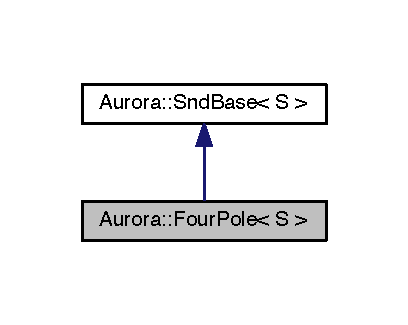
\includegraphics[width=196pt]{class_aurora_1_1_four_pole__inherit__graph}
\end{center}
\end{figure}


Collaboration diagram for Aurora\+:\+:Four\+Pole$<$ S $>$\+:\nopagebreak
\begin{figure}[H]
\begin{center}
\leavevmode
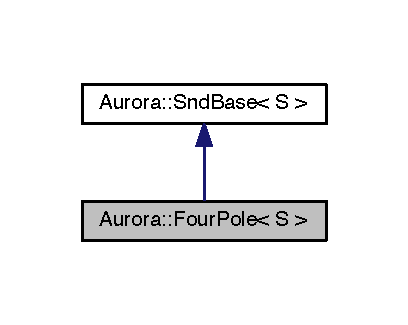
\includegraphics[width=196pt]{class_aurora_1_1_four_pole__coll__graph}
\end{center}
\end{figure}
\subsection*{Public Member Functions}
\begin{DoxyCompactItemize}
\item 
\hyperlink{class_aurora_1_1_four_pole_acd6f1e5b94bdc248e8e955f4ef8f7dcc}{Four\+Pole} (S sr=\hyperlink{namespace_aurora_ad49263d809bea98dd422e95bc91bc03e}{def\+\_\+sr}, int \hyperlink{class_aurora_1_1_snd_base_af9e21aaf411b17f7a8221c991ce5d291}{vsize}=\hyperlink{namespace_aurora_afaaddf667a06e7ce23c667a8b7295263}{def\+\_\+vsize})
\item 
const std\+::vector$<$ S $>$ \& \hyperlink{class_aurora_1_1_four_pole_ac3cfee8b5d8f0bf8d0b0c6784eb81fef}{operator()} (const std\+::vector$<$ S $>$ \&in, S f, S r)
\item 
const std\+::vector$<$ S $>$ \& \hyperlink{class_aurora_1_1_four_pole_a300ec87b54b5e8c5c76c1005fe31c9d9}{operator()} (const std\+::vector$<$ S $>$ \&in, const std\+::vector$<$ S $>$ \&f, S r)
\item 
void \hyperlink{class_aurora_1_1_four_pole_a5de080ccd74617a6bfba13d3d76bcb4b}{reset} (S fs)
\end{DoxyCompactItemize}


\subsection{Detailed Description}
\subsubsection*{template$<$typename S$>$\newline
class Aurora\+::\+Four\+Pole$<$ S $>$}

\hyperlink{class_aurora_1_1_four_pole}{Four\+Pole} class ~\newline
4-\/pole lowpass filter ~\newline
S\+: sample type 

\subsection{Constructor \& Destructor Documentation}
\mbox{\Hypertarget{class_aurora_1_1_four_pole_acd6f1e5b94bdc248e8e955f4ef8f7dcc}\label{class_aurora_1_1_four_pole_acd6f1e5b94bdc248e8e955f4ef8f7dcc}} 
\index{Aurora\+::\+Four\+Pole@{Aurora\+::\+Four\+Pole}!Four\+Pole@{Four\+Pole}}
\index{Four\+Pole@{Four\+Pole}!Aurora\+::\+Four\+Pole@{Aurora\+::\+Four\+Pole}}
\subsubsection{\texorpdfstring{Four\+Pole()}{FourPole()}}
{\footnotesize\ttfamily template$<$typename S $>$ \\
\hyperlink{class_aurora_1_1_four_pole}{Aurora\+::\+Four\+Pole}$<$ S $>$\+::\hyperlink{class_aurora_1_1_four_pole}{Four\+Pole} (\begin{DoxyParamCaption}\item[{S}]{sr = {\ttfamily \hyperlink{namespace_aurora_ad49263d809bea98dd422e95bc91bc03e}{def\+\_\+sr}},  }\item[{int}]{vsize = {\ttfamily \hyperlink{namespace_aurora_afaaddf667a06e7ce23c667a8b7295263}{def\+\_\+vsize}} }\end{DoxyParamCaption})\hspace{0.3cm}{\ttfamily [inline]}}

Constructor ~\newline
sr\+: sampling rate ~\newline
vsize\+: vector size 

\subsection{Member Function Documentation}
\mbox{\Hypertarget{class_aurora_1_1_four_pole_ac3cfee8b5d8f0bf8d0b0c6784eb81fef}\label{class_aurora_1_1_four_pole_ac3cfee8b5d8f0bf8d0b0c6784eb81fef}} 
\index{Aurora\+::\+Four\+Pole@{Aurora\+::\+Four\+Pole}!operator()@{operator()}}
\index{operator()@{operator()}!Aurora\+::\+Four\+Pole@{Aurora\+::\+Four\+Pole}}
\subsubsection{\texorpdfstring{operator()()}{operator()()}\hspace{0.1cm}{\footnotesize\ttfamily [1/2]}}
{\footnotesize\ttfamily template$<$typename S $>$ \\
const std\+::vector$<$S$>$\& \hyperlink{class_aurora_1_1_four_pole}{Aurora\+::\+Four\+Pole}$<$ S $>$\+::operator() (\begin{DoxyParamCaption}\item[{const std\+::vector$<$ S $>$ \&}]{in,  }\item[{S}]{f,  }\item[{S}]{r }\end{DoxyParamCaption})\hspace{0.3cm}{\ttfamily [inline]}}

Filter ~\newline
in\+: input ~\newline
f\+: cutoff frequency ~\newline
r\+: resonance (0-\/1) \mbox{\Hypertarget{class_aurora_1_1_four_pole_a300ec87b54b5e8c5c76c1005fe31c9d9}\label{class_aurora_1_1_four_pole_a300ec87b54b5e8c5c76c1005fe31c9d9}} 
\index{Aurora\+::\+Four\+Pole@{Aurora\+::\+Four\+Pole}!operator()@{operator()}}
\index{operator()@{operator()}!Aurora\+::\+Four\+Pole@{Aurora\+::\+Four\+Pole}}
\subsubsection{\texorpdfstring{operator()()}{operator()()}\hspace{0.1cm}{\footnotesize\ttfamily [2/2]}}
{\footnotesize\ttfamily template$<$typename S $>$ \\
const std\+::vector$<$S$>$\& \hyperlink{class_aurora_1_1_four_pole}{Aurora\+::\+Four\+Pole}$<$ S $>$\+::operator() (\begin{DoxyParamCaption}\item[{const std\+::vector$<$ S $>$ \&}]{in,  }\item[{const std\+::vector$<$ S $>$ \&}]{f,  }\item[{S}]{r }\end{DoxyParamCaption})\hspace{0.3cm}{\ttfamily [inline]}}

Filter ~\newline
in\+: input ~\newline
f\+: cutoff frequency ~\newline
r\+: resonance (0-\/1) \mbox{\Hypertarget{class_aurora_1_1_four_pole_a5de080ccd74617a6bfba13d3d76bcb4b}\label{class_aurora_1_1_four_pole_a5de080ccd74617a6bfba13d3d76bcb4b}} 
\index{Aurora\+::\+Four\+Pole@{Aurora\+::\+Four\+Pole}!reset@{reset}}
\index{reset@{reset}!Aurora\+::\+Four\+Pole@{Aurora\+::\+Four\+Pole}}
\subsubsection{\texorpdfstring{reset()}{reset()}}
{\footnotesize\ttfamily template$<$typename S $>$ \\
void \hyperlink{class_aurora_1_1_four_pole}{Aurora\+::\+Four\+Pole}$<$ S $>$\+::reset (\begin{DoxyParamCaption}\item[{S}]{fs }\end{DoxyParamCaption})\hspace{0.3cm}{\ttfamily [inline]}}

reset the filter ~\newline
fs\+: sampling rate 

The documentation for this class was generated from the following file\+:\begin{DoxyCompactItemize}
\item 
\hyperlink{_four_pole_8h}{Four\+Pole.\+h}\end{DoxyCompactItemize}

\hypertarget{class_aurora_1_1_osc}{}\section{Aurora\+:\+:Osc$<$ S $>$ Class Template Reference}
\label{class_aurora_1_1_osc}\index{Aurora\+::\+Osc$<$ S $>$@{Aurora\+::\+Osc$<$ S $>$}}


{\ttfamily \#include $<$Osc.\+h$>$}



Inheritance diagram for Aurora\+:\+:Osc$<$ S $>$\+:
\nopagebreak
\begin{figure}[H]
\begin{center}
\leavevmode
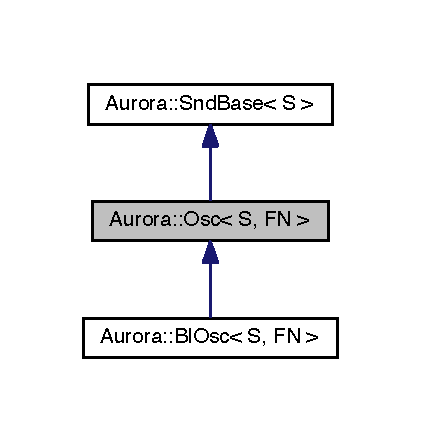
\includegraphics[width=196pt]{class_aurora_1_1_osc__inherit__graph}
\end{center}
\end{figure}


Collaboration diagram for Aurora\+:\+:Osc$<$ S $>$\+:
\nopagebreak
\begin{figure}[H]
\begin{center}
\leavevmode
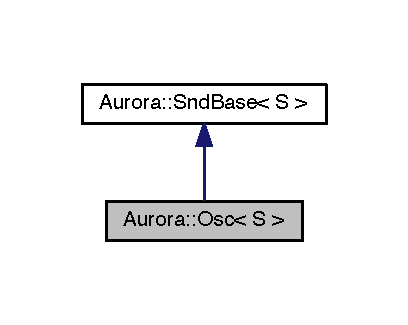
\includegraphics[width=196pt]{class_aurora_1_1_osc__coll__graph}
\end{center}
\end{figure}
\subsection*{Public Member Functions}
\begin{DoxyCompactItemize}
\item 
\hyperlink{class_aurora_1_1_osc_aca573068f8919635cfca278c7b087e38}{Osc} (const std\+::function$<$ S(S)$>$ f=\hyperlink{namespace_aurora_ab6ef1b966b8f27d107fcabe1027a677a}{cos}$<$ S $>$, S \hyperlink{class_aurora_1_1_osc_a9ac3aa9006fc98588b2163e0e56f6e30}{fs}=(S) \hyperlink{namespace_aurora_ad49263d809bea98dd422e95bc91bc03e}{def\+\_\+sr}, std\+::size\+\_\+t \hyperlink{class_aurora_1_1_snd_base_af9e21aaf411b17f7a8221c991ce5d291}{vsize}=\hyperlink{namespace_aurora_afaaddf667a06e7ce23c667a8b7295263}{def\+\_\+vsize})
\item 
virtual \hyperlink{class_aurora_1_1_osc_a95062ac1670f5de00a27c33bfb4eb117}{$\sim$\+Osc} ()
\item 
S \hyperlink{class_aurora_1_1_osc_a9ac3aa9006fc98588b2163e0e56f6e30}{fs} () const
\item 
const std\+::vector$<$ S $>$ \& \hyperlink{class_aurora_1_1_osc_a2a36c0afda86b6fabad4ed3ca0f510af}{operator()} (S a, S f)
\item 
const std\+::vector$<$ S $>$ \& \hyperlink{class_aurora_1_1_osc_af48611ef63363221de325d8976a1ec56}{operator()} (S a, const std\+::vector$<$ S $>$ \&fm)
\item 
const std\+::vector$<$ S $>$ \& \hyperlink{class_aurora_1_1_osc_a28fe97e5634b8a02474657ed456c326b}{operator()} (const std\+::vector$<$ S $>$ \&am, S f)
\item 
const std\+::vector$<$ S $>$ \& \hyperlink{class_aurora_1_1_osc_a06f9ead5fbf828f7ebb8617ac6cb24b4}{operator()} (const std\+::vector$<$ S $>$ \&am, const std\+::vector$<$ S $>$ \&fm)
\item 
const std\+::vector$<$ S $>$ \& \hyperlink{class_aurora_1_1_osc_a21019c4df8f4cf26af9fc50ac0c9f336}{operator()} (S a, S f, const std\+::vector$<$ S $>$ \&pm)
\item 
const std\+::vector$<$ S $>$ \& \hyperlink{class_aurora_1_1_osc_a6a8967d1e19757d77521e5b64842f7e3}{operator()} (const std\+::vector$<$ S $>$ \&am, S f, const std\+::vector$<$ S $>$ \&pm)
\item 
void \hyperlink{class_aurora_1_1_osc_a47029d701edea820aba145788b6f5bb6}{func} (const std\+::function$<$ S(S)$>$ f)
\item 
void \hyperlink{class_aurora_1_1_osc_a5828ab7fc7bddc7d8f4e349844f220b3}{phase} (double phs)
\item 
void \hyperlink{class_aurora_1_1_osc_a74abc44400ec00c9ff1dad13cdb24000}{reset} (S \hyperlink{class_aurora_1_1_osc_a9ac3aa9006fc98588b2163e0e56f6e30}{fs})
\item 
\hyperlink{class_aurora_1_1_osc_a5d145d20c6cef19473680c3ff5e1a874}{Osc} (const std\+::vector$<$ S $>$ $\ast$t=nullptr, S \hyperlink{class_aurora_1_1_osc_a9ac3aa9006fc98588b2163e0e56f6e30}{fs}=(S) \hyperlink{namespace_aurora_ad49263d809bea98dd422e95bc91bc03e}{def\+\_\+sr}, std\+::size\+\_\+t \hyperlink{class_aurora_1_1_snd_base_af9e21aaf411b17f7a8221c991ce5d291}{vsize}=\hyperlink{namespace_aurora_afaaddf667a06e7ce23c667a8b7295263}{def\+\_\+vsize})
\item 
virtual \hyperlink{class_aurora_1_1_osc_a95062ac1670f5de00a27c33bfb4eb117}{$\sim$\+Osc} ()
\item 
S \hyperlink{class_aurora_1_1_osc_a9ac3aa9006fc98588b2163e0e56f6e30}{fs} () const
\item 
const std\+::vector$<$ S $>$ \& \hyperlink{class_aurora_1_1_osc_a2a36c0afda86b6fabad4ed3ca0f510af}{operator()} (S a, S f)
\item 
const std\+::vector$<$ S $>$ \& \hyperlink{class_aurora_1_1_osc_af48611ef63363221de325d8976a1ec56}{operator()} (S a, const std\+::vector$<$ S $>$ \&fm)
\item 
const std\+::vector$<$ S $>$ \& \hyperlink{class_aurora_1_1_osc_a28fe97e5634b8a02474657ed456c326b}{operator()} (const std\+::vector$<$ S $>$ \&am, S f)
\item 
const std\+::vector$<$ S $>$ \& \hyperlink{class_aurora_1_1_osc_a06f9ead5fbf828f7ebb8617ac6cb24b4}{operator()} (const std\+::vector$<$ S $>$ \&am, const std\+::vector$<$ S $>$ \&fm)
\item 
const std\+::vector$<$ S $>$ \& \hyperlink{class_aurora_1_1_osc_a21019c4df8f4cf26af9fc50ac0c9f336}{operator()} (S a, S f, const std\+::vector$<$ S $>$ \&pm)
\item 
const std\+::vector$<$ S $>$ \& \hyperlink{class_aurora_1_1_osc_a6a8967d1e19757d77521e5b64842f7e3}{operator()} (const std\+::vector$<$ S $>$ \&am, S f, const std\+::vector$<$ S $>$ \&pm)
\item 
void \hyperlink{class_aurora_1_1_osc_a5828ab7fc7bddc7d8f4e349844f220b3}{phase} (double phs)
\item 
void \hyperlink{class_aurora_1_1_osc_a74abc44400ec00c9ff1dad13cdb24000}{reset} (S \hyperlink{class_aurora_1_1_osc_a9ac3aa9006fc98588b2163e0e56f6e30}{fs})
\end{DoxyCompactItemize}


\subsection{Detailed Description}
\subsubsection*{template$<$typename S$>$\newline
class Aurora\+::\+Osc$<$ S $>$}

\hyperlink{class_aurora_1_1_osc}{Osc} class ~\newline
Generic oscillator ~\newline
S\+: sample type

\hyperlink{class_aurora_1_1_osc}{Osc} class ~\newline
Generic templated oscillator ~\newline
S\+: sample type ~\newline
FN\+: oscillator function 

\subsection{Constructor \& Destructor Documentation}
\mbox{\Hypertarget{class_aurora_1_1_osc_aca573068f8919635cfca278c7b087e38}\label{class_aurora_1_1_osc_aca573068f8919635cfca278c7b087e38}} 
\index{Aurora\+::\+Osc@{Aurora\+::\+Osc}!Osc@{Osc}}
\index{Osc@{Osc}!Aurora\+::\+Osc@{Aurora\+::\+Osc}}
\subsubsection{\texorpdfstring{Osc()}{Osc()}\hspace{0.1cm}{\footnotesize\ttfamily [1/2]}}
{\footnotesize\ttfamily template$<$typename S$>$ \\
\hyperlink{class_aurora_1_1_osc}{Aurora\+::\+Osc}$<$ S $>$\+::\hyperlink{class_aurora_1_1_osc}{Osc} (\begin{DoxyParamCaption}\item[{const std\+::function$<$ S(S)$>$}]{f = {\ttfamily \hyperlink{namespace_aurora_ab6ef1b966b8f27d107fcabe1027a677a}{cos}$<$S$>$},  }\item[{S}]{fs = {\ttfamily (S)\hyperlink{namespace_aurora_ad49263d809bea98dd422e95bc91bc03e}{def\+\_\+sr}},  }\item[{std\+::size\+\_\+t}]{vsize = {\ttfamily \hyperlink{namespace_aurora_afaaddf667a06e7ce23c667a8b7295263}{def\+\_\+vsize}} }\end{DoxyParamCaption})\hspace{0.3cm}{\ttfamily [inline]}}

Constructor ~\newline
f\+: oscillator function ~\newline
fs\+: sampling rate ~\newline
vsize\+: signal vector size \mbox{\Hypertarget{class_aurora_1_1_osc_a95062ac1670f5de00a27c33bfb4eb117}\label{class_aurora_1_1_osc_a95062ac1670f5de00a27c33bfb4eb117}} 
\index{Aurora\+::\+Osc@{Aurora\+::\+Osc}!````~Osc@{$\sim$\+Osc}}
\index{````~Osc@{$\sim$\+Osc}!Aurora\+::\+Osc@{Aurora\+::\+Osc}}
\subsubsection{\texorpdfstring{$\sim$\+Osc()}{~Osc()}\hspace{0.1cm}{\footnotesize\ttfamily [1/2]}}
{\footnotesize\ttfamily template$<$typename S$>$ \\
virtual \hyperlink{class_aurora_1_1_osc}{Aurora\+::\+Osc}$<$ S $>$\+::$\sim$\hyperlink{class_aurora_1_1_osc}{Osc} (\begin{DoxyParamCaption}{ }\end{DoxyParamCaption})\hspace{0.3cm}{\ttfamily [inline]}, {\ttfamily [virtual]}}

\mbox{\Hypertarget{class_aurora_1_1_osc_a5d145d20c6cef19473680c3ff5e1a874}\label{class_aurora_1_1_osc_a5d145d20c6cef19473680c3ff5e1a874}} 
\index{Aurora\+::\+Osc@{Aurora\+::\+Osc}!Osc@{Osc}}
\index{Osc@{Osc}!Aurora\+::\+Osc@{Aurora\+::\+Osc}}
\subsubsection{\texorpdfstring{Osc()}{Osc()}\hspace{0.1cm}{\footnotesize\ttfamily [2/2]}}
{\footnotesize\ttfamily template$<$typename S$>$ \\
\hyperlink{class_aurora_1_1_osc}{Aurora\+::\+Osc}$<$ S $>$\+::\hyperlink{class_aurora_1_1_osc}{Osc} (\begin{DoxyParamCaption}\item[{const std\+::vector$<$ S $>$ $\ast$}]{t = {\ttfamily nullptr},  }\item[{S}]{fs = {\ttfamily (S)\hyperlink{namespace_aurora_ad49263d809bea98dd422e95bc91bc03e}{def\+\_\+sr}},  }\item[{std\+::size\+\_\+t}]{vsize = {\ttfamily \hyperlink{namespace_aurora_afaaddf667a06e7ce23c667a8b7295263}{def\+\_\+vsize}} }\end{DoxyParamCaption})\hspace{0.3cm}{\ttfamily [inline]}}

Constructor ~\newline
f\+: oscillator function ~\newline
fs\+: sampling rate ~\newline
vsize\+: signal vector size \mbox{\Hypertarget{class_aurora_1_1_osc_a95062ac1670f5de00a27c33bfb4eb117}\label{class_aurora_1_1_osc_a95062ac1670f5de00a27c33bfb4eb117}} 
\index{Aurora\+::\+Osc@{Aurora\+::\+Osc}!````~Osc@{$\sim$\+Osc}}
\index{````~Osc@{$\sim$\+Osc}!Aurora\+::\+Osc@{Aurora\+::\+Osc}}
\subsubsection{\texorpdfstring{$\sim$\+Osc()}{~Osc()}\hspace{0.1cm}{\footnotesize\ttfamily [2/2]}}
{\footnotesize\ttfamily template$<$typename S$>$ \\
virtual \hyperlink{class_aurora_1_1_osc}{Aurora\+::\+Osc}$<$ S $>$\+::$\sim$\hyperlink{class_aurora_1_1_osc}{Osc} (\begin{DoxyParamCaption}{ }\end{DoxyParamCaption})\hspace{0.3cm}{\ttfamily [inline]}, {\ttfamily [virtual]}}



\subsection{Member Function Documentation}
\mbox{\Hypertarget{class_aurora_1_1_osc_a9ac3aa9006fc98588b2163e0e56f6e30}\label{class_aurora_1_1_osc_a9ac3aa9006fc98588b2163e0e56f6e30}} 
\index{Aurora\+::\+Osc@{Aurora\+::\+Osc}!fs@{fs}}
\index{fs@{fs}!Aurora\+::\+Osc@{Aurora\+::\+Osc}}
\subsubsection{\texorpdfstring{fs()}{fs()}\hspace{0.1cm}{\footnotesize\ttfamily [1/2]}}
{\footnotesize\ttfamily template$<$typename S$>$ \\
S \hyperlink{class_aurora_1_1_osc}{Aurora\+::\+Osc}$<$ S $>$\+::fs (\begin{DoxyParamCaption}{ }\end{DoxyParamCaption}) const\hspace{0.3cm}{\ttfamily [inline]}}

Sampling rate query ~\newline
returns sampling rate \mbox{\Hypertarget{class_aurora_1_1_osc_a9ac3aa9006fc98588b2163e0e56f6e30}\label{class_aurora_1_1_osc_a9ac3aa9006fc98588b2163e0e56f6e30}} 
\index{Aurora\+::\+Osc@{Aurora\+::\+Osc}!fs@{fs}}
\index{fs@{fs}!Aurora\+::\+Osc@{Aurora\+::\+Osc}}
\subsubsection{\texorpdfstring{fs()}{fs()}\hspace{0.1cm}{\footnotesize\ttfamily [2/2]}}
{\footnotesize\ttfamily template$<$typename S$>$ \\
S \hyperlink{class_aurora_1_1_osc}{Aurora\+::\+Osc}$<$ S $>$\+::fs (\begin{DoxyParamCaption}{ }\end{DoxyParamCaption}) const\hspace{0.3cm}{\ttfamily [inline]}}

Sampling rate query ~\newline
returns sampling rate \mbox{\Hypertarget{class_aurora_1_1_osc_a47029d701edea820aba145788b6f5bb6}\label{class_aurora_1_1_osc_a47029d701edea820aba145788b6f5bb6}} 
\index{Aurora\+::\+Osc@{Aurora\+::\+Osc}!func@{func}}
\index{func@{func}!Aurora\+::\+Osc@{Aurora\+::\+Osc}}
\subsubsection{\texorpdfstring{func()}{func()}}
{\footnotesize\ttfamily template$<$typename S$>$ \\
void \hyperlink{class_aurora_1_1_osc}{Aurora\+::\+Osc}$<$ S $>$\+::func (\begin{DoxyParamCaption}\item[{const std\+::function$<$ S(S)$>$}]{f }\end{DoxyParamCaption})\hspace{0.3cm}{\ttfamily [inline]}}

set the oscillator function ~\newline
f\+: oscillator function to be used \mbox{\Hypertarget{class_aurora_1_1_osc_a2a36c0afda86b6fabad4ed3ca0f510af}\label{class_aurora_1_1_osc_a2a36c0afda86b6fabad4ed3ca0f510af}} 
\index{Aurora\+::\+Osc@{Aurora\+::\+Osc}!operator()@{operator()}}
\index{operator()@{operator()}!Aurora\+::\+Osc@{Aurora\+::\+Osc}}
\subsubsection{\texorpdfstring{operator()()}{operator()()}\hspace{0.1cm}{\footnotesize\ttfamily [1/12]}}
{\footnotesize\ttfamily template$<$typename S$>$ \\
const std\+::vector$<$S$>$\& \hyperlink{class_aurora_1_1_osc}{Aurora\+::\+Osc}$<$ S $>$\+::operator() (\begin{DoxyParamCaption}\item[{S}]{a,  }\item[{S}]{f }\end{DoxyParamCaption})\hspace{0.3cm}{\ttfamily [inline]}}

Oscillator ~\newline
a\+: scalar amplitude ~\newline
f\+: scalar frequency ~\newline
returns reference to object signal vector \mbox{\Hypertarget{class_aurora_1_1_osc_af48611ef63363221de325d8976a1ec56}\label{class_aurora_1_1_osc_af48611ef63363221de325d8976a1ec56}} 
\index{Aurora\+::\+Osc@{Aurora\+::\+Osc}!operator()@{operator()}}
\index{operator()@{operator()}!Aurora\+::\+Osc@{Aurora\+::\+Osc}}
\subsubsection{\texorpdfstring{operator()()}{operator()()}\hspace{0.1cm}{\footnotesize\ttfamily [2/12]}}
{\footnotesize\ttfamily template$<$typename S$>$ \\
const std\+::vector$<$S$>$\& \hyperlink{class_aurora_1_1_osc}{Aurora\+::\+Osc}$<$ S $>$\+::operator() (\begin{DoxyParamCaption}\item[{S}]{a,  }\item[{const std\+::vector$<$ S $>$ \&}]{fm }\end{DoxyParamCaption})\hspace{0.3cm}{\ttfamily [inline]}}

Oscillator ~\newline
a\+: scalar amplitude ~\newline
fm\+: frequency signal ~\newline
returns reference to object signal vector \mbox{\Hypertarget{class_aurora_1_1_osc_a2a36c0afda86b6fabad4ed3ca0f510af}\label{class_aurora_1_1_osc_a2a36c0afda86b6fabad4ed3ca0f510af}} 
\index{Aurora\+::\+Osc@{Aurora\+::\+Osc}!operator()@{operator()}}
\index{operator()@{operator()}!Aurora\+::\+Osc@{Aurora\+::\+Osc}}
\subsubsection{\texorpdfstring{operator()()}{operator()()}\hspace{0.1cm}{\footnotesize\ttfamily [3/12]}}
{\footnotesize\ttfamily template$<$typename S$>$ \\
const std\+::vector$<$S$>$\& \hyperlink{class_aurora_1_1_osc}{Aurora\+::\+Osc}$<$ S $>$\+::operator() (\begin{DoxyParamCaption}\item[{S}]{a,  }\item[{S}]{f }\end{DoxyParamCaption})\hspace{0.3cm}{\ttfamily [inline]}}

Oscillator ~\newline
a\+: scalar amplitude ~\newline
f\+: scalar frequency ~\newline
returns reference to object signal vector \mbox{\Hypertarget{class_aurora_1_1_osc_a28fe97e5634b8a02474657ed456c326b}\label{class_aurora_1_1_osc_a28fe97e5634b8a02474657ed456c326b}} 
\index{Aurora\+::\+Osc@{Aurora\+::\+Osc}!operator()@{operator()}}
\index{operator()@{operator()}!Aurora\+::\+Osc@{Aurora\+::\+Osc}}
\subsubsection{\texorpdfstring{operator()()}{operator()()}\hspace{0.1cm}{\footnotesize\ttfamily [4/12]}}
{\footnotesize\ttfamily template$<$typename S$>$ \\
const std\+::vector$<$S$>$\& \hyperlink{class_aurora_1_1_osc}{Aurora\+::\+Osc}$<$ S $>$\+::operator() (\begin{DoxyParamCaption}\item[{const std\+::vector$<$ S $>$ \&}]{am,  }\item[{S}]{f }\end{DoxyParamCaption})\hspace{0.3cm}{\ttfamily [inline]}}

Oscillator ~\newline
am\+: amplitude signal ~\newline
f\+: scalar frequency ~\newline
returns reference to object signal vector \mbox{\Hypertarget{class_aurora_1_1_osc_af48611ef63363221de325d8976a1ec56}\label{class_aurora_1_1_osc_af48611ef63363221de325d8976a1ec56}} 
\index{Aurora\+::\+Osc@{Aurora\+::\+Osc}!operator()@{operator()}}
\index{operator()@{operator()}!Aurora\+::\+Osc@{Aurora\+::\+Osc}}
\subsubsection{\texorpdfstring{operator()()}{operator()()}\hspace{0.1cm}{\footnotesize\ttfamily [5/12]}}
{\footnotesize\ttfamily template$<$typename S$>$ \\
const std\+::vector$<$S$>$\& \hyperlink{class_aurora_1_1_osc}{Aurora\+::\+Osc}$<$ S $>$\+::operator() (\begin{DoxyParamCaption}\item[{S}]{a,  }\item[{const std\+::vector$<$ S $>$ \&}]{fm }\end{DoxyParamCaption})\hspace{0.3cm}{\ttfamily [inline]}}

Oscillator ~\newline
a\+: scalar amplitude ~\newline
fm\+: frequency signal ~\newline
returns reference to object signal vector \mbox{\Hypertarget{class_aurora_1_1_osc_a06f9ead5fbf828f7ebb8617ac6cb24b4}\label{class_aurora_1_1_osc_a06f9ead5fbf828f7ebb8617ac6cb24b4}} 
\index{Aurora\+::\+Osc@{Aurora\+::\+Osc}!operator()@{operator()}}
\index{operator()@{operator()}!Aurora\+::\+Osc@{Aurora\+::\+Osc}}
\subsubsection{\texorpdfstring{operator()()}{operator()()}\hspace{0.1cm}{\footnotesize\ttfamily [6/12]}}
{\footnotesize\ttfamily template$<$typename S$>$ \\
const std\+::vector$<$S$>$\& \hyperlink{class_aurora_1_1_osc}{Aurora\+::\+Osc}$<$ S $>$\+::operator() (\begin{DoxyParamCaption}\item[{const std\+::vector$<$ S $>$ \&}]{am,  }\item[{const std\+::vector$<$ S $>$ \&}]{fm }\end{DoxyParamCaption})\hspace{0.3cm}{\ttfamily [inline]}}

Oscillator ~\newline
am\+: amplitude signal ~\newline
fm\+: frequency signal ~\newline
returns reference to object signal vector \mbox{\Hypertarget{class_aurora_1_1_osc_a28fe97e5634b8a02474657ed456c326b}\label{class_aurora_1_1_osc_a28fe97e5634b8a02474657ed456c326b}} 
\index{Aurora\+::\+Osc@{Aurora\+::\+Osc}!operator()@{operator()}}
\index{operator()@{operator()}!Aurora\+::\+Osc@{Aurora\+::\+Osc}}
\subsubsection{\texorpdfstring{operator()()}{operator()()}\hspace{0.1cm}{\footnotesize\ttfamily [7/12]}}
{\footnotesize\ttfamily template$<$typename S$>$ \\
const std\+::vector$<$S$>$\& \hyperlink{class_aurora_1_1_osc}{Aurora\+::\+Osc}$<$ S $>$\+::operator() (\begin{DoxyParamCaption}\item[{const std\+::vector$<$ S $>$ \&}]{am,  }\item[{S}]{f }\end{DoxyParamCaption})\hspace{0.3cm}{\ttfamily [inline]}}

Oscillator ~\newline
am\+: amplitude signal ~\newline
f\+: scalar frequency ~\newline
returns reference to object signal vector \mbox{\Hypertarget{class_aurora_1_1_osc_a06f9ead5fbf828f7ebb8617ac6cb24b4}\label{class_aurora_1_1_osc_a06f9ead5fbf828f7ebb8617ac6cb24b4}} 
\index{Aurora\+::\+Osc@{Aurora\+::\+Osc}!operator()@{operator()}}
\index{operator()@{operator()}!Aurora\+::\+Osc@{Aurora\+::\+Osc}}
\subsubsection{\texorpdfstring{operator()()}{operator()()}\hspace{0.1cm}{\footnotesize\ttfamily [8/12]}}
{\footnotesize\ttfamily template$<$typename S$>$ \\
const std\+::vector$<$S$>$\& \hyperlink{class_aurora_1_1_osc}{Aurora\+::\+Osc}$<$ S $>$\+::operator() (\begin{DoxyParamCaption}\item[{const std\+::vector$<$ S $>$ \&}]{am,  }\item[{const std\+::vector$<$ S $>$ \&}]{fm }\end{DoxyParamCaption})\hspace{0.3cm}{\ttfamily [inline]}}

Oscillator ~\newline
am\+: amplitude signal ~\newline
fm\+: frequency signal ~\newline
returns reference to object signal vector \mbox{\Hypertarget{class_aurora_1_1_osc_a21019c4df8f4cf26af9fc50ac0c9f336}\label{class_aurora_1_1_osc_a21019c4df8f4cf26af9fc50ac0c9f336}} 
\index{Aurora\+::\+Osc@{Aurora\+::\+Osc}!operator()@{operator()}}
\index{operator()@{operator()}!Aurora\+::\+Osc@{Aurora\+::\+Osc}}
\subsubsection{\texorpdfstring{operator()()}{operator()()}\hspace{0.1cm}{\footnotesize\ttfamily [9/12]}}
{\footnotesize\ttfamily template$<$typename S$>$ \\
const std\+::vector$<$S$>$\& \hyperlink{class_aurora_1_1_osc}{Aurora\+::\+Osc}$<$ S $>$\+::operator() (\begin{DoxyParamCaption}\item[{S}]{a,  }\item[{S}]{f,  }\item[{const std\+::vector$<$ S $>$ \&}]{pm }\end{DoxyParamCaption})\hspace{0.3cm}{\ttfamily [inline]}}

Oscillator ~\newline
 a\+: scalar amplitude ~\newline
f\+: scalar frequency ~\newline
pm\+: phase modulation signal ~\newline
returns reference to object signal vector \mbox{\Hypertarget{class_aurora_1_1_osc_a21019c4df8f4cf26af9fc50ac0c9f336}\label{class_aurora_1_1_osc_a21019c4df8f4cf26af9fc50ac0c9f336}} 
\index{Aurora\+::\+Osc@{Aurora\+::\+Osc}!operator()@{operator()}}
\index{operator()@{operator()}!Aurora\+::\+Osc@{Aurora\+::\+Osc}}
\subsubsection{\texorpdfstring{operator()()}{operator()()}\hspace{0.1cm}{\footnotesize\ttfamily [10/12]}}
{\footnotesize\ttfamily template$<$typename S$>$ \\
const std\+::vector$<$S$>$\& \hyperlink{class_aurora_1_1_osc}{Aurora\+::\+Osc}$<$ S $>$\+::operator() (\begin{DoxyParamCaption}\item[{S}]{a,  }\item[{S}]{f,  }\item[{const std\+::vector$<$ S $>$ \&}]{pm }\end{DoxyParamCaption})\hspace{0.3cm}{\ttfamily [inline]}}

Oscillator ~\newline
a\+: scalar amplitude ~\newline
f\+: scalar frequency ~\newline
pm\+: phase modulation signal ~\newline
returns reference to object signal vector \mbox{\Hypertarget{class_aurora_1_1_osc_a6a8967d1e19757d77521e5b64842f7e3}\label{class_aurora_1_1_osc_a6a8967d1e19757d77521e5b64842f7e3}} 
\index{Aurora\+::\+Osc@{Aurora\+::\+Osc}!operator()@{operator()}}
\index{operator()@{operator()}!Aurora\+::\+Osc@{Aurora\+::\+Osc}}
\subsubsection{\texorpdfstring{operator()()}{operator()()}\hspace{0.1cm}{\footnotesize\ttfamily [11/12]}}
{\footnotesize\ttfamily template$<$typename S$>$ \\
const std\+::vector$<$S$>$\& \hyperlink{class_aurora_1_1_osc}{Aurora\+::\+Osc}$<$ S $>$\+::operator() (\begin{DoxyParamCaption}\item[{const std\+::vector$<$ S $>$ \&}]{am,  }\item[{S}]{f,  }\item[{const std\+::vector$<$ S $>$ \&}]{pm }\end{DoxyParamCaption})\hspace{0.3cm}{\ttfamily [inline]}}

Oscillator ~\newline
am\+: amplitude signal ~\newline
f\+: scalar frequency ~\newline
pm\+: phase modulation signal ~\newline
returns reference to object signal vector \mbox{\Hypertarget{class_aurora_1_1_osc_a6a8967d1e19757d77521e5b64842f7e3}\label{class_aurora_1_1_osc_a6a8967d1e19757d77521e5b64842f7e3}} 
\index{Aurora\+::\+Osc@{Aurora\+::\+Osc}!operator()@{operator()}}
\index{operator()@{operator()}!Aurora\+::\+Osc@{Aurora\+::\+Osc}}
\subsubsection{\texorpdfstring{operator()()}{operator()()}\hspace{0.1cm}{\footnotesize\ttfamily [12/12]}}
{\footnotesize\ttfamily template$<$typename S$>$ \\
const std\+::vector$<$S$>$\& \hyperlink{class_aurora_1_1_osc}{Aurora\+::\+Osc}$<$ S $>$\+::operator() (\begin{DoxyParamCaption}\item[{const std\+::vector$<$ S $>$ \&}]{am,  }\item[{S}]{f,  }\item[{const std\+::vector$<$ S $>$ \&}]{pm }\end{DoxyParamCaption})\hspace{0.3cm}{\ttfamily [inline]}}

Oscillator ~\newline
am\+: amplitude signal ~\newline
f\+: scalar frequency ~\newline
pm\+: phase modulation signal ~\newline
returns reference to object signal vector \mbox{\Hypertarget{class_aurora_1_1_osc_a5828ab7fc7bddc7d8f4e349844f220b3}\label{class_aurora_1_1_osc_a5828ab7fc7bddc7d8f4e349844f220b3}} 
\index{Aurora\+::\+Osc@{Aurora\+::\+Osc}!phase@{phase}}
\index{phase@{phase}!Aurora\+::\+Osc@{Aurora\+::\+Osc}}
\subsubsection{\texorpdfstring{phase()}{phase()}\hspace{0.1cm}{\footnotesize\ttfamily [1/2]}}
{\footnotesize\ttfamily template$<$typename S$>$ \\
void \hyperlink{class_aurora_1_1_osc}{Aurora\+::\+Osc}$<$ S $>$\+::phase (\begin{DoxyParamCaption}\item[{double}]{phs }\end{DoxyParamCaption})\hspace{0.3cm}{\ttfamily [inline]}}

set the internal oscillator phase ~\newline
phs\+: phase \mbox{\Hypertarget{class_aurora_1_1_osc_a5828ab7fc7bddc7d8f4e349844f220b3}\label{class_aurora_1_1_osc_a5828ab7fc7bddc7d8f4e349844f220b3}} 
\index{Aurora\+::\+Osc@{Aurora\+::\+Osc}!phase@{phase}}
\index{phase@{phase}!Aurora\+::\+Osc@{Aurora\+::\+Osc}}
\subsubsection{\texorpdfstring{phase()}{phase()}\hspace{0.1cm}{\footnotesize\ttfamily [2/2]}}
{\footnotesize\ttfamily template$<$typename S$>$ \\
void \hyperlink{class_aurora_1_1_osc}{Aurora\+::\+Osc}$<$ S $>$\+::phase (\begin{DoxyParamCaption}\item[{double}]{phs }\end{DoxyParamCaption})\hspace{0.3cm}{\ttfamily [inline]}}

set the internal oscillator phase ~\newline
phs\+: phase \mbox{\Hypertarget{class_aurora_1_1_osc_a74abc44400ec00c9ff1dad13cdb24000}\label{class_aurora_1_1_osc_a74abc44400ec00c9ff1dad13cdb24000}} 
\index{Aurora\+::\+Osc@{Aurora\+::\+Osc}!reset@{reset}}
\index{reset@{reset}!Aurora\+::\+Osc@{Aurora\+::\+Osc}}
\subsubsection{\texorpdfstring{reset()}{reset()}\hspace{0.1cm}{\footnotesize\ttfamily [1/2]}}
{\footnotesize\ttfamily template$<$typename S$>$ \\
void \hyperlink{class_aurora_1_1_osc}{Aurora\+::\+Osc}$<$ S $>$\+::reset (\begin{DoxyParamCaption}\item[{S}]{fs }\end{DoxyParamCaption})\hspace{0.3cm}{\ttfamily [inline]}}

reset the oscillator ~\newline
fs\+: sampling rate \mbox{\Hypertarget{class_aurora_1_1_osc_a74abc44400ec00c9ff1dad13cdb24000}\label{class_aurora_1_1_osc_a74abc44400ec00c9ff1dad13cdb24000}} 
\index{Aurora\+::\+Osc@{Aurora\+::\+Osc}!reset@{reset}}
\index{reset@{reset}!Aurora\+::\+Osc@{Aurora\+::\+Osc}}
\subsubsection{\texorpdfstring{reset()}{reset()}\hspace{0.1cm}{\footnotesize\ttfamily [2/2]}}
{\footnotesize\ttfamily template$<$typename S$>$ \\
void \hyperlink{class_aurora_1_1_osc}{Aurora\+::\+Osc}$<$ S $>$\+::reset (\begin{DoxyParamCaption}\item[{S}]{fs }\end{DoxyParamCaption})\hspace{0.3cm}{\ttfamily [inline]}}

reset the oscillator ~\newline
fs\+: sampling rate 

The documentation for this class was generated from the following files\+:\begin{DoxyCompactItemize}
\item 
\hyperlink{_osc_8h}{Osc.\+h}\item 
\hyperlink{_osc_t_8h}{Osc\+T.\+h}\end{DoxyCompactItemize}

\hypertarget{class_aurora_1_1_snd_base}{}\section{Aurora\+:\+:Snd\+Base$<$ S $>$ Class Template Reference}
\label{class_aurora_1_1_snd_base}\index{Aurora\+::\+Snd\+Base$<$ S $>$@{Aurora\+::\+Snd\+Base$<$ S $>$}}


{\ttfamily \#include $<$Snd\+Base.\+h$>$}



Inheritance diagram for Aurora\+:\+:Snd\+Base$<$ S $>$\+:
\nopagebreak
\begin{figure}[H]
\begin{center}
\leavevmode
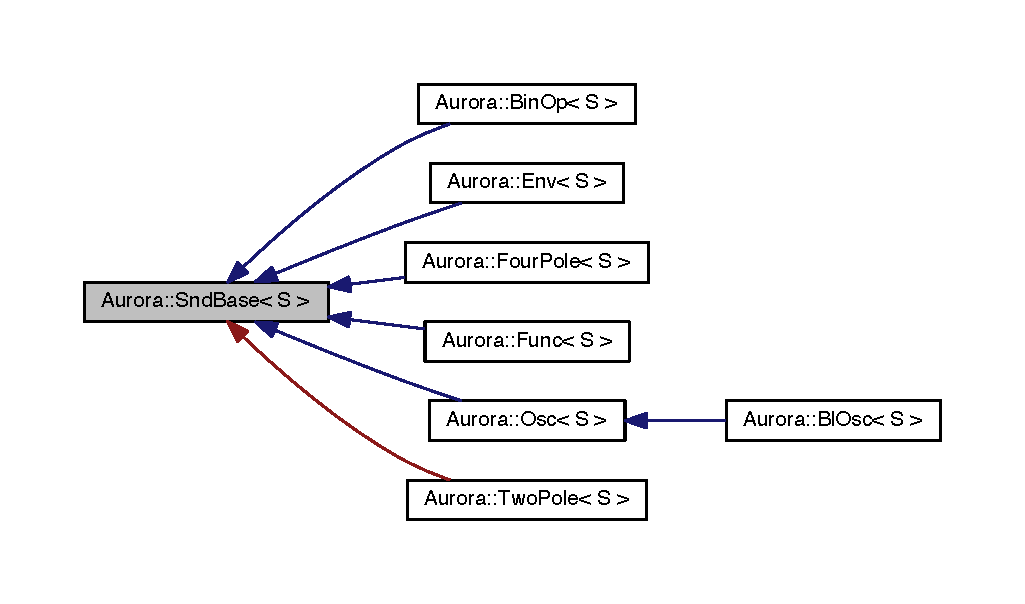
\includegraphics[width=350pt]{class_aurora_1_1_snd_base__inherit__graph}
\end{center}
\end{figure}
\subsection*{Public Member Functions}
\begin{DoxyCompactItemize}
\item 
\hyperlink{class_aurora_1_1_snd_base_a960739d3ae63df581c28f8801e589a3c}{Snd\+Base} (std\+::size\+\_\+t \hyperlink{class_aurora_1_1_snd_base_ad68387541cc3d696d0cf58d474f94b73}{vsize}=\hyperlink{namespace_aurora_afaaddf667a06e7ce23c667a8b7295263}{def\+\_\+vsize})
\item 
std\+::size\+\_\+t \hyperlink{class_aurora_1_1_snd_base_ad68387541cc3d696d0cf58d474f94b73}{vsize} ()
\item 
void \hyperlink{class_aurora_1_1_snd_base_a88dacba995eef179f2fc97e11a331913}{vsize} (std\+::size\+\_\+t n)
\item 
const std\+::vector$<$ S $>$ \& \hyperlink{class_aurora_1_1_snd_base_aecf7b916b5b459b5ac2855997fd2aec6}{vector} ()
\item 
void \hyperlink{class_aurora_1_1_snd_base_a5d57c3b735e5d583b4b4ae5f8e9cdf4c}{prealloc} (std\+::size\+\_\+t size)
\end{DoxyCompactItemize}
\subsection*{Protected Attributes}
\begin{DoxyCompactItemize}
\item 
std\+::vector$<$ S $>$ \hyperlink{class_aurora_1_1_snd_base_adad6cd3430a1510dc887cc6bd1a45658}{sig}
\end{DoxyCompactItemize}


\subsection{Detailed Description}
\subsubsection*{template$<$typename S$>$\newline
class Aurora\+::\+Snd\+Base$<$ S $>$}

\hyperlink{class_aurora_1_1_snd_base}{Snd\+Base} class ~\newline
\hyperlink{namespace_aurora}{Aurora} Library base class 

\subsection{Constructor \& Destructor Documentation}
\mbox{\Hypertarget{class_aurora_1_1_snd_base_a960739d3ae63df581c28f8801e589a3c}\label{class_aurora_1_1_snd_base_a960739d3ae63df581c28f8801e589a3c}} 
\index{Aurora\+::\+Snd\+Base@{Aurora\+::\+Snd\+Base}!Snd\+Base@{Snd\+Base}}
\index{Snd\+Base@{Snd\+Base}!Aurora\+::\+Snd\+Base@{Aurora\+::\+Snd\+Base}}
\subsubsection{\texorpdfstring{Snd\+Base()}{SndBase()}}
{\footnotesize\ttfamily template$<$typename S $>$ \\
\hyperlink{class_aurora_1_1_snd_base}{Aurora\+::\+Snd\+Base}$<$ S $>$\+::\hyperlink{class_aurora_1_1_snd_base}{Snd\+Base} (\begin{DoxyParamCaption}\item[{std\+::size\+\_\+t}]{vsize = {\ttfamily \hyperlink{namespace_aurora_afaaddf667a06e7ce23c667a8b7295263}{def\+\_\+vsize}} }\end{DoxyParamCaption})\hspace{0.3cm}{\ttfamily [inline]}}

Constructor ~\newline
vsize\+: signal vector size 

\subsection{Member Function Documentation}
\mbox{\Hypertarget{class_aurora_1_1_snd_base_a5d57c3b735e5d583b4b4ae5f8e9cdf4c}\label{class_aurora_1_1_snd_base_a5d57c3b735e5d583b4b4ae5f8e9cdf4c}} 
\index{Aurora\+::\+Snd\+Base@{Aurora\+::\+Snd\+Base}!prealloc@{prealloc}}
\index{prealloc@{prealloc}!Aurora\+::\+Snd\+Base@{Aurora\+::\+Snd\+Base}}
\subsubsection{\texorpdfstring{prealloc()}{prealloc()}}
{\footnotesize\ttfamily template$<$typename S $>$ \\
void \hyperlink{class_aurora_1_1_snd_base}{Aurora\+::\+Snd\+Base}$<$ S $>$\+::prealloc (\begin{DoxyParamCaption}\item[{std\+::size\+\_\+t}]{size }\end{DoxyParamCaption})\hspace{0.3cm}{\ttfamily [inline]}}

Preallocate vector memory ~\newline
size\+: size of vector to reserve in memory ~\newline
this method does not change the vector size. \mbox{\Hypertarget{class_aurora_1_1_snd_base_aecf7b916b5b459b5ac2855997fd2aec6}\label{class_aurora_1_1_snd_base_aecf7b916b5b459b5ac2855997fd2aec6}} 
\index{Aurora\+::\+Snd\+Base@{Aurora\+::\+Snd\+Base}!vector@{vector}}
\index{vector@{vector}!Aurora\+::\+Snd\+Base@{Aurora\+::\+Snd\+Base}}
\subsubsection{\texorpdfstring{vector()}{vector()}}
{\footnotesize\ttfamily template$<$typename S $>$ \\
const std\+::vector$<$S$>$\& \hyperlink{class_aurora_1_1_snd_base}{Aurora\+::\+Snd\+Base}$<$ S $>$\+::vector (\begin{DoxyParamCaption}{ }\end{DoxyParamCaption})\hspace{0.3cm}{\ttfamily [inline]}}

Vector access ~\newline
returns the object vector \mbox{\Hypertarget{class_aurora_1_1_snd_base_ad68387541cc3d696d0cf58d474f94b73}\label{class_aurora_1_1_snd_base_ad68387541cc3d696d0cf58d474f94b73}} 
\index{Aurora\+::\+Snd\+Base@{Aurora\+::\+Snd\+Base}!vsize@{vsize}}
\index{vsize@{vsize}!Aurora\+::\+Snd\+Base@{Aurora\+::\+Snd\+Base}}
\subsubsection{\texorpdfstring{vsize()}{vsize()}\hspace{0.1cm}{\footnotesize\ttfamily [1/2]}}
{\footnotesize\ttfamily template$<$typename S $>$ \\
std\+::size\+\_\+t \hyperlink{class_aurora_1_1_snd_base}{Aurora\+::\+Snd\+Base}$<$ S $>$\+::vsize (\begin{DoxyParamCaption}{ }\end{DoxyParamCaption})\hspace{0.3cm}{\ttfamily [inline]}}

Vector size query ~\newline
returns the object vector size \mbox{\Hypertarget{class_aurora_1_1_snd_base_a88dacba995eef179f2fc97e11a331913}\label{class_aurora_1_1_snd_base_a88dacba995eef179f2fc97e11a331913}} 
\index{Aurora\+::\+Snd\+Base@{Aurora\+::\+Snd\+Base}!vsize@{vsize}}
\index{vsize@{vsize}!Aurora\+::\+Snd\+Base@{Aurora\+::\+Snd\+Base}}
\subsubsection{\texorpdfstring{vsize()}{vsize()}\hspace{0.1cm}{\footnotesize\ttfamily [2/2]}}
{\footnotesize\ttfamily template$<$typename S $>$ \\
void \hyperlink{class_aurora_1_1_snd_base}{Aurora\+::\+Snd\+Base}$<$ S $>$\+::vsize (\begin{DoxyParamCaption}\item[{std\+::size\+\_\+t}]{n }\end{DoxyParamCaption})\hspace{0.3cm}{\ttfamily [inline]}}

Vector size setting ~\newline
n\+: new vector size 

\subsection{Member Data Documentation}
\mbox{\Hypertarget{class_aurora_1_1_snd_base_adad6cd3430a1510dc887cc6bd1a45658}\label{class_aurora_1_1_snd_base_adad6cd3430a1510dc887cc6bd1a45658}} 
\index{Aurora\+::\+Snd\+Base@{Aurora\+::\+Snd\+Base}!sig@{sig}}
\index{sig@{sig}!Aurora\+::\+Snd\+Base@{Aurora\+::\+Snd\+Base}}
\subsubsection{\texorpdfstring{sig}{sig}}
{\footnotesize\ttfamily template$<$typename S $>$ \\
std\+::vector$<$S$>$ \hyperlink{class_aurora_1_1_snd_base}{Aurora\+::\+Snd\+Base}$<$ S $>$\+::sig\hspace{0.3cm}{\ttfamily [protected]}}



The documentation for this class was generated from the following file\+:\begin{DoxyCompactItemize}
\item 
\hyperlink{_snd_base_8h}{Snd\+Base.\+h}\end{DoxyCompactItemize}

\hypertarget{class_aurora_1_1_table_set}{}\section{Aurora\+:\+:Table\+Set$<$ S $>$ Class Template Reference}
\label{class_aurora_1_1_table_set}\index{Aurora\+::\+Table\+Set$<$ S $>$@{Aurora\+::\+Table\+Set$<$ S $>$}}


{\ttfamily \#include $<$Bl\+Osc.\+h$>$}

\subsection*{Public Member Functions}
\begin{DoxyCompactItemize}
\item 
\hyperlink{class_aurora_1_1_table_set_a0be4528b972606335d73ac312da6337b}{Table\+Set} (uint32\+\_\+t type, S fs=\hyperlink{namespace_aurora_ad49263d809bea98dd422e95bc91bc03e}{def\+\_\+sr}, std\+::size\+\_\+t len=\hyperlink{namespace_aurora_a14dabfd9feedfa09c0e6f86d2627f006}{def\+\_\+ftlen})
\item 
\hyperlink{class_aurora_1_1_table_set_a884ecfde480fdac4c32fa10a82286941}{Table\+Set} (const std\+::vector$<$ S $>$ \&src, S b=\hyperlink{namespace_aurora_acb267dff62f74484893c2d5b679b78bf}{def\+\_\+base}, S fs=\hyperlink{namespace_aurora_ad49263d809bea98dd422e95bc91bc03e}{def\+\_\+sr})
\item 
std\+::function$<$ S(S)$>$ \hyperlink{class_aurora_1_1_table_set_a27a325a2c3c4b8cd50e0c86d6ac3c617}{func} (S f) const
\end{DoxyCompactItemize}


\subsection{Detailed Description}
\subsubsection*{template$<$typename S$>$\newline
class Aurora\+::\+Table\+Set$<$ S $>$}

\hyperlink{class_aurora_1_1_table_set}{Table\+Set} class ~\newline
Creates a set of tables for \hyperlink{class_aurora_1_1_bl_osc}{Bl\+Osc}. ~\newline
S\+: sample type 

\subsection{Constructor \& Destructor Documentation}
\mbox{\Hypertarget{class_aurora_1_1_table_set_a0be4528b972606335d73ac312da6337b}\label{class_aurora_1_1_table_set_a0be4528b972606335d73ac312da6337b}} 
\index{Aurora\+::\+Table\+Set@{Aurora\+::\+Table\+Set}!Table\+Set@{Table\+Set}}
\index{Table\+Set@{Table\+Set}!Aurora\+::\+Table\+Set@{Aurora\+::\+Table\+Set}}
\subsubsection{\texorpdfstring{Table\+Set()}{TableSet()}\hspace{0.1cm}{\footnotesize\ttfamily [1/2]}}
{\footnotesize\ttfamily template$<$typename S$>$ \\
\hyperlink{class_aurora_1_1_table_set}{Aurora\+::\+Table\+Set}$<$ S $>$\+::\hyperlink{class_aurora_1_1_table_set}{Table\+Set} (\begin{DoxyParamCaption}\item[{uint32\+\_\+t}]{type,  }\item[{S}]{fs = {\ttfamily \hyperlink{namespace_aurora_ad49263d809bea98dd422e95bc91bc03e}{def\+\_\+sr}},  }\item[{std\+::size\+\_\+t}]{len = {\ttfamily \hyperlink{namespace_aurora_a14dabfd9feedfa09c0e6f86d2627f006}{def\+\_\+ftlen}} }\end{DoxyParamCaption})\hspace{0.3cm}{\ttfamily [inline]}}

Constructor ~\newline
type\+: wave type (S\+AW, S\+Q\+U\+A\+RE, T\+R\+I\+A\+N\+G\+LE, P\+U\+L\+SE) ~\newline
fs\+: sampling rate for which these will be built ~\newline
len\+: table length \mbox{\Hypertarget{class_aurora_1_1_table_set_a884ecfde480fdac4c32fa10a82286941}\label{class_aurora_1_1_table_set_a884ecfde480fdac4c32fa10a82286941}} 
\index{Aurora\+::\+Table\+Set@{Aurora\+::\+Table\+Set}!Table\+Set@{Table\+Set}}
\index{Table\+Set@{Table\+Set}!Aurora\+::\+Table\+Set@{Aurora\+::\+Table\+Set}}
\subsubsection{\texorpdfstring{Table\+Set()}{TableSet()}\hspace{0.1cm}{\footnotesize\ttfamily [2/2]}}
{\footnotesize\ttfamily template$<$typename S$>$ \\
\hyperlink{class_aurora_1_1_table_set}{Aurora\+::\+Table\+Set}$<$ S $>$\+::\hyperlink{class_aurora_1_1_table_set}{Table\+Set} (\begin{DoxyParamCaption}\item[{const std\+::vector$<$ S $>$ \&}]{src,  }\item[{S}]{b = {\ttfamily \hyperlink{namespace_aurora_acb267dff62f74484893c2d5b679b78bf}{def\+\_\+base}},  }\item[{S}]{fs = {\ttfamily \hyperlink{namespace_aurora_ad49263d809bea98dd422e95bc91bc03e}{def\+\_\+sr}} }\end{DoxyParamCaption})\hspace{0.3cm}{\ttfamily [inline]}}

Constructor ~\newline
src\+: source wave table ~\newline
b\+: base frequency for wavetables ~\newline
octs\+: number of octaves to generate ~\newline
fs\+: sampling rate for which these will be built 

\subsection{Member Function Documentation}
\mbox{\Hypertarget{class_aurora_1_1_table_set_a27a325a2c3c4b8cd50e0c86d6ac3c617}\label{class_aurora_1_1_table_set_a27a325a2c3c4b8cd50e0c86d6ac3c617}} 
\index{Aurora\+::\+Table\+Set@{Aurora\+::\+Table\+Set}!func@{func}}
\index{func@{func}!Aurora\+::\+Table\+Set@{Aurora\+::\+Table\+Set}}
\subsubsection{\texorpdfstring{func()}{func()}}
{\footnotesize\ttfamily template$<$typename S$>$ \\
std\+::function$<$S(S)$>$ \hyperlink{class_aurora_1_1_table_set}{Aurora\+::\+Table\+Set}$<$ S $>$\+::func (\begin{DoxyParamCaption}\item[{S}]{f }\end{DoxyParamCaption}) const\hspace{0.3cm}{\ttfamily [inline]}}

Function selection ~\newline
f\+: fundamental frequency used for playback 

The documentation for this class was generated from the following file\+:\begin{DoxyCompactItemize}
\item 
\hyperlink{_bl_osc_8h}{Bl\+Osc.\+h}\end{DoxyCompactItemize}

\chapter{File Documentation}
\hypertarget{_bl_osc_8h}{}\section{Bl\+Osc.\+h File Reference}
\label{_bl_osc_8h}\index{Bl\+Osc.\+h@{Bl\+Osc.\+h}}
{\ttfamily \#include \char`\"{}F\+F\+T.\+h\char`\"{}}\newline
{\ttfamily \#include \char`\"{}Osc.\+h\char`\"{}}\newline
Include dependency graph for Bl\+Osc.\+h\+:
\nopagebreak
\begin{figure}[H]
\begin{center}
\leavevmode
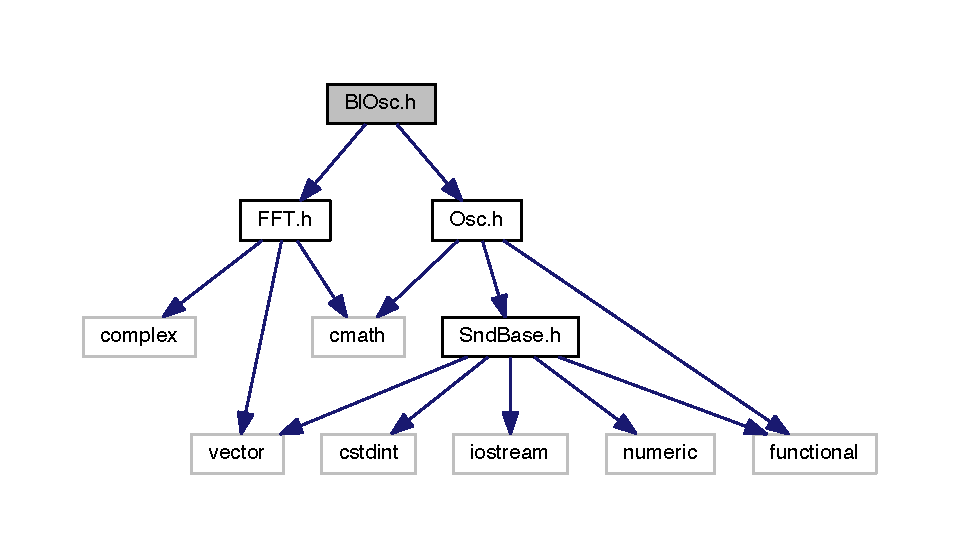
\includegraphics[width=350pt]{_bl_osc_8h__incl}
\end{center}
\end{figure}
\subsection*{Classes}
\begin{DoxyCompactItemize}
\item 
class \hyperlink{class_aurora_1_1_table_set}{Aurora\+::\+Table\+Set$<$ S $>$}
\item 
class \hyperlink{class_aurora_1_1_bl_osc}{Aurora\+::\+Bl\+Osc$<$ S, F\+N $>$}
\end{DoxyCompactItemize}
\subsection*{Namespaces}
\begin{DoxyCompactItemize}
\item 
 \hyperlink{namespace_aurora}{Aurora}
\end{DoxyCompactItemize}
\subsection*{Enumerations}
\begin{DoxyCompactItemize}
\item 
enum \{ \hyperlink{namespace_aurora_a890b8d3786c8a25750e8097adae3b513ad47a607309b6d737bba699a295e5e814}{Aurora\+::\+S\+AW} = 0, 
\hyperlink{namespace_aurora_a890b8d3786c8a25750e8097adae3b513ad12f117b00f964cb4de3809ca2e2fa2b}{Aurora\+::\+S\+Q\+U\+A\+RE}, 
\hyperlink{namespace_aurora_a890b8d3786c8a25750e8097adae3b513a0c9e1e4fb03cbc79bb5fdd9db743818f}{Aurora\+::\+T\+R\+I\+A\+N\+G\+LE}, 
\hyperlink{namespace_aurora_a890b8d3786c8a25750e8097adae3b513aa52ebfb9f31c0d7f0da3f2f66b622928}{Aurora\+::\+P\+U\+L\+SE}
 \}
\end{DoxyCompactItemize}
\subsection*{Variables}
\begin{DoxyCompactItemize}
\item 
const double \hyperlink{namespace_aurora_acb267dff62f74484893c2d5b679b78bf}{Aurora\+::def\+\_\+base} = 16.
\item 
const int \hyperlink{namespace_aurora_a14dabfd9feedfa09c0e6f86d2627f006}{Aurora\+::def\+\_\+ftlen} = 16384
\end{DoxyCompactItemize}

\hypertarget{_env_8h}{}\section{Env.\+h File Reference}
\label{_env_8h}\index{Env.\+h@{Env.\+h}}
{\ttfamily \#include \char`\"{}Snd\+Base.\+h\char`\"{}}\newline
{\ttfamily \#include $<$functional$>$}\newline
Include dependency graph for Env.\+h\+:
\nopagebreak
\begin{figure}[H]
\begin{center}
\leavevmode
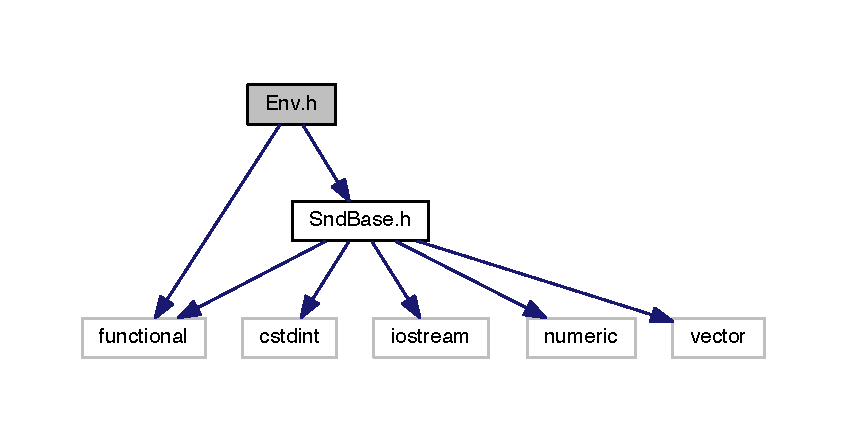
\includegraphics[width=350pt]{_env_8h__incl}
\end{center}
\end{figure}
\subsection*{Classes}
\begin{DoxyCompactItemize}
\item 
class \hyperlink{class_aurora_1_1_env}{Aurora\+::\+Env$<$ S, F\+N $>$}
\end{DoxyCompactItemize}
\subsection*{Namespaces}
\begin{DoxyCompactItemize}
\item 
 \hyperlink{namespace_aurora}{Aurora}
\end{DoxyCompactItemize}
\subsection*{Functions}
\begin{DoxyCompactItemize}
\item 
{\footnotesize template$<$typename S $>$ }\\S \hyperlink{namespace_aurora_a787aaa0540c8f3be97e0ad55ba643b0a}{Aurora\+::ads} (S a, S d, S s, double t, S e, S ts)
\item 
{\footnotesize template$<$typename S $>$ }\\std\+::function$<$ S(double, S, S)$>$ \hyperlink{namespace_aurora_aeac34405f4d58ec77eb9519844518255}{Aurora\+::env\+\_\+gen} (const std\+::vector$<$ S $>$ \&pts)
\item 
{\footnotesize template$<$typename S $>$ }\\std\+::function$<$ S(double, S, S)$>$ \hyperlink{namespace_aurora_ac7d13365b103aa497998c2bb23ad7f13}{Aurora\+::ads\+\_\+gen} (const S \&a, const S \&d, const S \&s)
\end{DoxyCompactItemize}

\hypertarget{_f_f_t_8h}{}\section{F\+F\+T.\+h File Reference}
\label{_f_f_t_8h}\index{F\+F\+T.\+h@{F\+F\+T.\+h}}
{\ttfamily \#include $<$cmath$>$}\newline
{\ttfamily \#include $<$complex$>$}\newline
{\ttfamily \#include $<$vector$>$}\newline
Include dependency graph for F\+F\+T.\+h\+:
\nopagebreak
\begin{figure}[H]
\begin{center}
\leavevmode
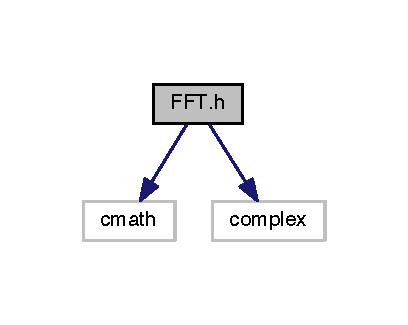
\includegraphics[width=258pt]{_f_f_t_8h__incl}
\end{center}
\end{figure}
This graph shows which files directly or indirectly include this file\+:
\nopagebreak
\begin{figure}[H]
\begin{center}
\leavevmode
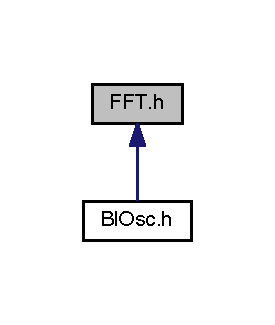
\includegraphics[width=198pt]{_f_f_t_8h__dep__incl}
\end{center}
\end{figure}
\subsection*{Classes}
\begin{DoxyCompactItemize}
\item 
class \hyperlink{class_aurora_1_1_f_f_t}{Aurora\+::\+F\+F\+T$<$ S $>$}
\end{DoxyCompactItemize}
\subsection*{Namespaces}
\begin{DoxyCompactItemize}
\item 
 \hyperlink{namespace_aurora}{Aurora}
\end{DoxyCompactItemize}
\subsection*{Macros}
\begin{DoxyCompactItemize}
\item 
\#define \hyperlink{_f_f_t_8h_ae71449b1cc6e6250b91f539153a7a0d3}{M\+\_\+\+PI}~3.\+14159265358979323846
\end{DoxyCompactItemize}
\subsection*{Functions}
\begin{DoxyCompactItemize}
\item 
static uint32\+\_\+t \hyperlink{namespace_aurora_a49b6f6d92479d80271ced42627154066}{Aurora\+::np2} (uint32\+\_\+t n)
\end{DoxyCompactItemize}
\subsection*{Variables}
\begin{DoxyCompactItemize}
\item 
const bool \hyperlink{namespace_aurora_a3e70ffc9ea5c526dcd66b1b14e43f175}{Aurora\+::packed} = true
\item 
static bool \hyperlink{namespace_aurora_a20b1bd3f1b34b8676e26d07718dac352}{Aurora\+::forward} = true
\item 
static bool \hyperlink{namespace_aurora_ac22c4e2e10572cbb6f64f3bd1cd595b5}{Aurora\+::inverse} = false
\end{DoxyCompactItemize}


\subsection{Macro Definition Documentation}
\mbox{\Hypertarget{_f_f_t_8h_ae71449b1cc6e6250b91f539153a7a0d3}\label{_f_f_t_8h_ae71449b1cc6e6250b91f539153a7a0d3}} 
\index{F\+F\+T.\+h@{F\+F\+T.\+h}!M\+\_\+\+PI@{M\+\_\+\+PI}}
\index{M\+\_\+\+PI@{M\+\_\+\+PI}!F\+F\+T.\+h@{F\+F\+T.\+h}}
\subsubsection{\texorpdfstring{M\+\_\+\+PI}{M\_PI}}
{\footnotesize\ttfamily \#define M\+\_\+\+PI~3.\+14159265358979323846}


\hypertarget{_four_pole_8h}{}\doxysection{Four\+Pole.\+h File Reference}
\label{_four_pole_8h}\index{FourPole.h@{FourPole.h}}
{\ttfamily \#include \char`\"{}Snd\+Base.\+h\char`\"{}}\newline
{\ttfamily \#include $<$cmath$>$}\newline
Include dependency graph for Four\+Pole.\+h\+:
\nopagebreak
\begin{figure}[H]
\begin{center}
\leavevmode
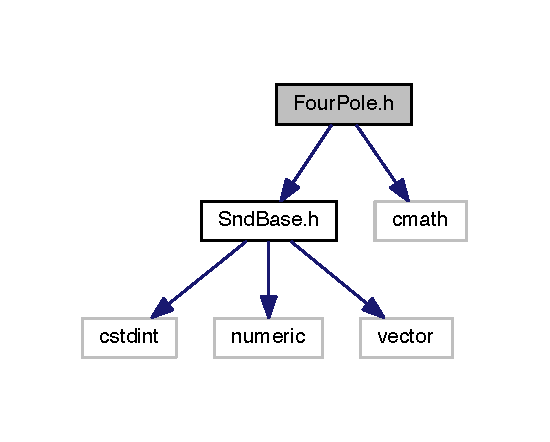
\includegraphics[width=350pt]{_four_pole_8h__incl}
\end{center}
\end{figure}
\doxysubsection*{Classes}
\begin{DoxyCompactItemize}
\item 
class \mbox{\hyperlink{class_aurora_1_1_four_pole}{Aurora\+::\+Four\+Pole$<$ S $>$}}
\end{DoxyCompactItemize}
\doxysubsection*{Namespaces}
\begin{DoxyCompactItemize}
\item 
namespace \mbox{\hyperlink{namespace_aurora}{Aurora}}
\end{DoxyCompactItemize}

\hypertarget{_osc_8h}{}\section{Osc.\+h File Reference}
\label{_osc_8h}\index{Osc.\+h@{Osc.\+h}}
{\ttfamily \#include \char`\"{}Snd\+Base.\+h\char`\"{}}\newline
{\ttfamily \#include $<$cmath$>$}\newline
{\ttfamily \#include $<$functional$>$}\newline
Include dependency graph for Osc.\+h\+:\nopagebreak
\begin{figure}[H]
\begin{center}
\leavevmode
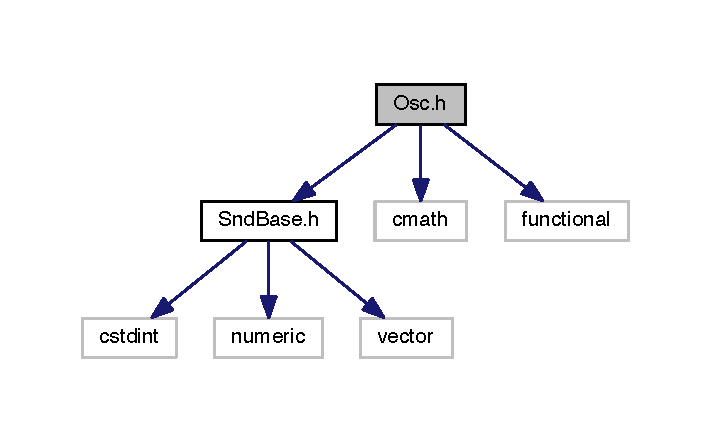
\includegraphics[width=350pt]{_osc_8h__incl}
\end{center}
\end{figure}
This graph shows which files directly or indirectly include this file\+:\nopagebreak
\begin{figure}[H]
\begin{center}
\leavevmode
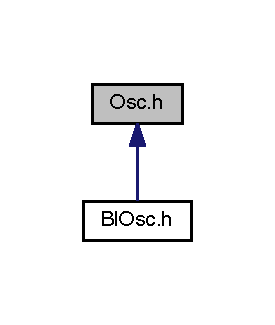
\includegraphics[width=132pt]{_osc_8h__dep__incl}
\end{center}
\end{figure}
\subsection*{Classes}
\begin{DoxyCompactItemize}
\item 
class \hyperlink{class_aurora_1_1_osc}{Aurora\+::\+Osc$<$ S, F\+N $>$}
\end{DoxyCompactItemize}
\subsection*{Namespaces}
\begin{DoxyCompactItemize}
\item 
 \hyperlink{namespace_aurora}{Aurora}
\end{DoxyCompactItemize}
\subsection*{Functions}
\begin{DoxyCompactItemize}
\item 
{\footnotesize template$<$typename S $>$ }\\S \hyperlink{namespace_aurora_ae0082f7bc3946a88145d54bacd0c6ff3}{Aurora\+::lookup} (double ph, const std\+::vector$<$ S $>$ $\ast$t)
\item 
{\footnotesize template$<$typename S $>$ }\\S \hyperlink{namespace_aurora_a9246ac499667da52a0d1750e5238c4a8}{Aurora\+::lookupi} (double ph, const std\+::vector$<$ S $>$ $\ast$t)
\item 
{\footnotesize template$<$typename S $>$ }\\S \hyperlink{namespace_aurora_afab81d7b8873e7850073124fcf37eeea}{Aurora\+::lookupc} (double ph, const std\+::vector$<$ S $>$ $\ast$t)
\item 
{\footnotesize template$<$typename S $>$ }\\S \hyperlink{namespace_aurora_a76909b8c5d5801213d35fffa69499885}{Aurora\+::sin} (double ph, const std\+::vector$<$ S $>$ $\ast$t=0)
\item 
{\footnotesize template$<$typename S $>$ }\\S \hyperlink{namespace_aurora_a0269c3758ab62d6a910cd8f7ace7fba2}{Aurora\+::cos} (double ph, const std\+::vector$<$ S $>$ $\ast$t=0)
\item 
{\footnotesize template$<$typename S $>$ }\\S \hyperlink{namespace_aurora_a6a6af5d9695d0ec8fcb343c456c1faab}{Aurora\+::phase} (double ph, const std\+::vector$<$ S $>$ $\ast$t=0)
\end{DoxyCompactItemize}
\subsection*{Variables}
\begin{DoxyCompactItemize}
\item 
const double \hyperlink{namespace_aurora_a4c08f8416c2b35d5001062f121459b5a}{Aurora\+::twopi} = 2 $\ast$ M\+\_\+\+PI
\item 
const int \hyperlink{namespace_aurora_a14dabfd9feedfa09c0e6f86d2627f006}{Aurora\+::def\+\_\+ftlen} = 16384
\end{DoxyCompactItemize}

\hypertarget{include_2_r_e_a_d_m_e_8md}{}\doxysection{README.\+md File Reference}
\label{include_2_r_e_a_d_m_e_8md}\index{README.md@{README.md}}

\hypertarget{_r_e_a_d_m_e_8md}{}\doxysection{README.\+md File Reference}
\label{_r_e_a_d_m_e_8md}\index{README.md@{README.md}}

\hypertarget{_snd_base_8h}{}\section{Snd\+Base.\+h File Reference}
\label{_snd_base_8h}\index{Snd\+Base.\+h@{Snd\+Base.\+h}}
{\ttfamily \#include $<$cstdint$>$}\newline
{\ttfamily \#include $<$numeric$>$}\newline
{\ttfamily \#include $<$vector$>$}\newline
Include dependency graph for Snd\+Base.\+h\+:\nopagebreak
\begin{figure}[H]
\begin{center}
\leavevmode
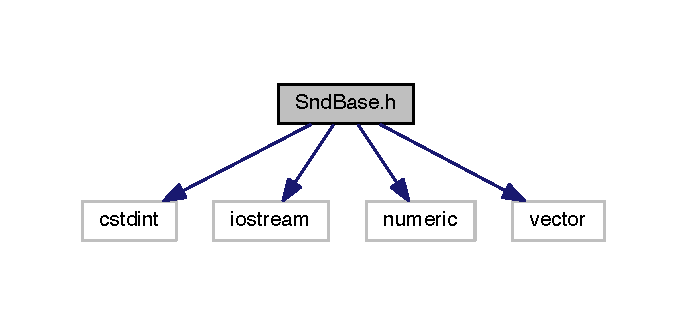
\includegraphics[width=257pt]{_snd_base_8h__incl}
\end{center}
\end{figure}
This graph shows which files directly or indirectly include this file\+:
\nopagebreak
\begin{figure}[H]
\begin{center}
\leavevmode
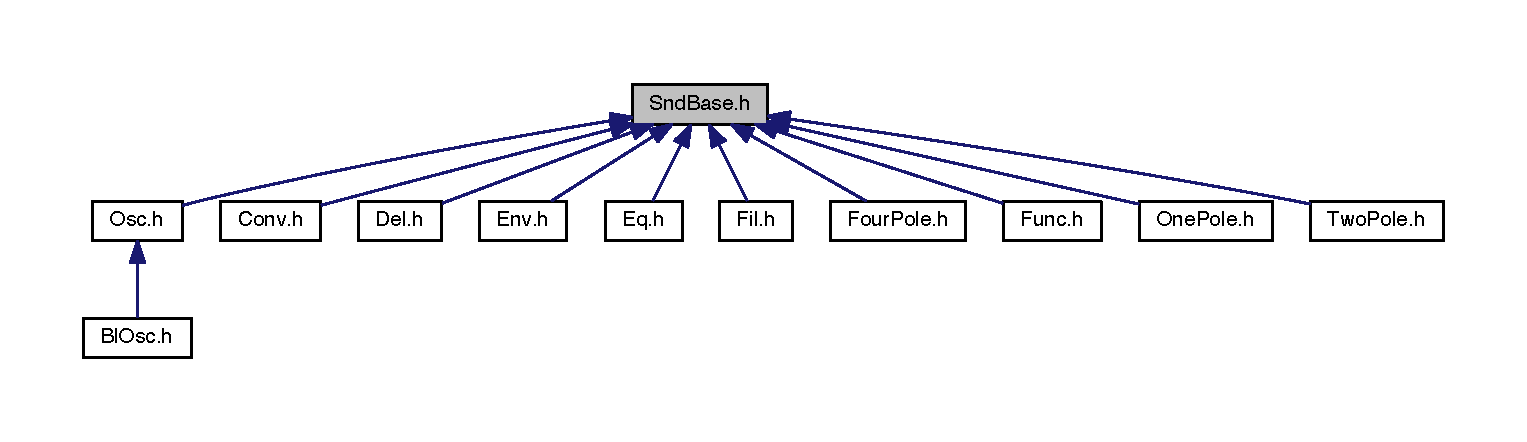
\includegraphics[width=336pt]{_snd_base_8h__dep__incl}
\end{center}
\end{figure}
\subsection*{Classes}
\begin{DoxyCompactItemize}
\item 
class \hyperlink{class_aurora_1_1_snd_base}{Aurora\+::\+Snd\+Base$<$ S $>$}
\item 
class \hyperlink{class_aurora_1_1_bin_op}{Aurora\+::\+Bin\+Op$<$ S $>$}
\end{DoxyCompactItemize}
\subsection*{Namespaces}
\begin{DoxyCompactItemize}
\item 
 \hyperlink{namespace_aurora}{Aurora}
\end{DoxyCompactItemize}
\subsection*{Variables}
\begin{DoxyCompactItemize}
\item 
const int \hyperlink{namespace_aurora_afaaddf667a06e7ce23c667a8b7295263}{Aurora\+::def\+\_\+vsize} = 64
\item 
const double \hyperlink{namespace_aurora_ad49263d809bea98dd422e95bc91bc03e}{Aurora\+::def\+\_\+sr} = 44100.
\end{DoxyCompactItemize}

%--- End generated contents ---

% Index
\backmatter
\newpage
\phantomsection
\clearemptydoublepage
\addcontentsline{toc}{chapter}{Index}
\printindex

\end{document}
